%%%%%%%%%%%%%%%%%%%%%%%%%%%%%%%%%%%%%%%%%
% Cleese Assignment (For Students)
% LaTeX Template
% Version 2.0 (27/5/2018)
%
% This template originates from:
% http://www.LaTeXTemplates.com
%
% Author:
% Vel (vel@LaTeXTemplates.com)
%
% License:
% CC BY-NC-SA 3.0 (http://creativecommons.org/licenses/by-nc-sa/3.0/)
% 
%%%%%%%%%%%%%%%%%%%%%%%%%%%%%%%%%%%%%%%%%

%----------------------------------------------------------------------------------------
%	PACKAGES AND OTHER DOCUMENT CONFIGURATIONS
%----------------------------------------------------------------------------------------

\documentclass[11pt]{article}
\usepackage{float}

%\usepackage[printwatermark]{xwatermark}
%\newwatermark[allpages,color=gray!50,angle=45,scale=2.5,xpos=-5,ypos=-5]{Mohammad Hadi}

%%%%%%%%%%%%%%%%%%%%%%%%%%%%%%%%%%%%%%%%%
% Cleese Assignment
% Structure Specification File
% Version 1.0 (27/5/2018)
%
% This template originates from:
% http://www.LaTeXTemplates.com
%
% Author:
% Vel (vel@LaTeXTemplates.com)
%
% License:
% CC BY-NC-SA 3.0 (http://creativecommons.org/licenses/by-nc-sa/3.0/)
% 
%%%%%%%%%%%%%%%%%%%%%%%%%%%%%%%%%%%%%%%%%

%----------------------------------------------------------------------------------------
%	PACKAGES AND OTHER DOCUMENT CONFIGURATIONS
%----------------------------------------------------------------------------------------

\usepackage{lastpage} % Required to determine the last page number for the footer

\usepackage{graphicx} % Required to insert images

\setlength\parindent{0pt} % Removes all indentation from paragraphs

\usepackage[most]{tcolorbox} % Required for boxes that split across pages

\usepackage{booktabs} % Required for better horizontal rules in tables

\usepackage{listings} % Required for insertion of code

\usepackage{etoolbox} % Required for if statements

%----------------------------------------------------------------------------------------
%	MARGINS
%----------------------------------------------------------------------------------------

\usepackage{geometry} % Required for adjusting page dimensions and margins

\geometry{
	paper=a4paper, % Change to letterpaper for US letter
	top=3cm, % Top margin
	bottom=3cm, % Bottom margin
	left=2.5cm, % Left margin
	right=2.5cm, % Right margin
	headheight=14pt, % Header height
	footskip=1.4cm, % Space from the bottom margin to the baseline of the footer
	headsep=1.2cm, % Space from the top margin to the baseline of the header
	%showframe, % Uncomment to show how the type block is set on the page
}

%----------------------------------------------------------------------------------------
%	FONT
%----------------------------------------------------------------------------------------

\usepackage[utf8]{inputenc} % Required for inputting international characters
\usepackage[T1]{fontenc} % Output font encoding for international characters

\usepackage[sfdefault,light]{roboto} % Use the Roboto font

%----------------------------------------------------------------------------------------
%	HEADERS AND FOOTERS
%----------------------------------------------------------------------------------------

\usepackage{fancyhdr} % Required for customising headers and footers

\pagestyle{fancy} % Enable custom headers and footers

\lhead{\small\assignmentClass\ifdef{\assignmentClassInstructor}{\ (\assignmentClassInstructor):}{}\ \assignmentTitle} % Left header; output the instructor in brackets if one was set
\chead{} % Centre header
\rhead{\small\ifdef{\assignmentAuthorName}{\assignmentAuthorName}{\ifdef{\assignmentDueDate}{Due\ \assignmentDueDate}{}}} % Right header; output the author name if one was set, otherwise the due date if that was set

\lfoot{} % Left footer
\cfoot{\small Page\ \thepage\ of\ \pageref{LastPage}} % Centre footer
\rfoot{} % Right footer

\renewcommand\headrulewidth{0.5pt} % Thickness of the header rule

%----------------------------------------------------------------------------------------
%	MODIFY SECTION STYLES
%----------------------------------------------------------------------------------------

\usepackage{titlesec} % Required for modifying sections

%------------------------------------------------
% Section

\titleformat
{\section} % Section type being modified
[block] % Shape type, can be: hang, block, display, runin, leftmargin, rightmargin, drop, wrap, frame
{\Large\bfseries} % Format of the whole section
{\assignmentQuestionName~\thesection} % Format of the section label
{6pt} % Space between the title and label
{} % Code before the label

\titlespacing{\section}{0pt}{0.5\baselineskip}{0.5\baselineskip} % Spacing around section titles, the order is: left, before and after

%------------------------------------------------
% Subsection

\titleformat
{\subsection} % Section type being modified
[block] % Shape type, can be: hang, block, display, runin, leftmargin, rightmargin, drop, wrap, frame
{\itshape} % Format of the whole section
{(\alph{subsection})} % Format of the section label
{4pt} % Space between the title and label
{} % Code before the label

\titlespacing{\subsection}{0pt}{0.5\baselineskip}{0.5\baselineskip} % Spacing around section titles, the order is: left, before and after

\renewcommand\thesubsection{(\alph{subsection})}

%----------------------------------------------------------------------------------------
%	CUSTOM QUESTION COMMANDS/ENVIRONMENTS
%----------------------------------------------------------------------------------------

% Environment to be used for each question in the assignment
\newenvironment{question}{
	\vspace{0.5\baselineskip} % Whitespace before the question
	\section{} % Blank section title (e.g. just Question 2)
	\lfoot{\small\itshape\assignmentQuestionName~\thesection~continued on next page\ldots} % Set the left footer to state the question continues on the next page, this is reset to nothing if it doesn't (below)
}{
	\lfoot{} % Reset the left footer to nothing if the current question does not continue on the next page
}

%------------------------------------------------

% Environment for subquestions, takes 1 argument - the name of the section
\newenvironment{subquestion}[1]{
	\subsection{#1}
}{
}

%------------------------------------------------

% Command to print a question sentence
\newcommand{\questiontext}[1]{
	\textbf{#1}
	\vspace{0.5\baselineskip} % Whitespace afterwards
}

%------------------------------------------------

% Command to print a box that breaks across pages with the question answer
\newcommand{\answer}[1]{
	\begin{tcolorbox}[breakable, enhanced]
		#1
	\end{tcolorbox}
}

%------------------------------------------------

% Command to print a box that breaks across pages with the space for a student to answer
\newcommand{\answerbox}[1]{
	\begin{tcolorbox}[breakable, enhanced]
		\vphantom{L}\vspace{\numexpr #1-1\relax\baselineskip} % \vphantom{L} to provide a typesetting strut with a height for the line, \numexpr to subtract user input by 1 to make it 0-based as this command is
	\end{tcolorbox}
}

%------------------------------------------------

% Command to print an assignment section title to split an assignment into major parts
\newcommand{\assignmentSection}[1]{
	{
		\centering % Centre the section title
		\vspace{2\baselineskip} % Whitespace before the entire section title
		
		\rule{0.8\textwidth}{0.5pt} % Horizontal rule
		
		\vspace{0.75\baselineskip} % Whitespace before the section title
		{\LARGE \MakeUppercase{#1}} % Section title, forced to be uppercase
		
		\rule{0.8\textwidth}{0.5pt} % Horizontal rule
		
		\vspace{\baselineskip} % Whitespace after the entire section title
	}
}

%----------------------------------------------------------------------------------------
%	TITLE PAGE
%----------------------------------------------------------------------------------------

\author{\textbf{\assignmentAuthorName}} % Set the default title page author field
\date{} % Don't use the default title page date field

\title{
	\thispagestyle{empty} % Suppress headers and footers
	\vspace{0.2\textheight} % Whitespace before the title
	\textbf{\assignmentClass:\ \assignmentTitle}\\[-4pt]
	\ifdef{\assignmentDueDate}{{\small Due\ on\ \assignmentDueDate}\\}{} % If a due date is supplied, output it
	\ifdef{\assignmentClassInstructor}{{\large \textit{\assignmentClassInstructor}}}{} % If an instructor is supplied, output it
	\vspace{0.32\textheight} % Whitespace before the author name
}
 % Include the file specifying the document structure and custom commands

%----------------------------------------------------------------------------------------
%	ASSIGNMENT INFORMATION
%----------------------------------------------------------------------------------------

% Required
\newcommand{\assignmentQuestionName}{Experiment} % The word to be used as a prefix to question numbers; example alternatives: Problem, Exercise
\newcommand{\assignmentClass}{Electrical Circuits Lab (Taught by Mohammad Hadi)\\Manual 2 (Due on DDD.,\ mmm.\ dd,\ yyyy)} % Course (Lecturer)\\Assignment (Due date)
\newcommand{\assignmentTitle}{} % Assignment title or name
\newcommand{\assignmentAuthorName}{Sina Hashemi \& M.Mahdi Shokrzade\\402102668 - 402101985} % Student name\\Student number
%----------------------------------------------------------------------------------------

\newcommand{\PicScale}{0.2}

\begin{document}
\textbf{Function generator is an electronic equipment used to generate different periodic electrical signals. DC power supply is an instrument that gives DC voltage to power a device. Multi-meter is a measuring instrument that can measure various electrical properties. In this experiment, you learn how to work with function generator, DC power supply, and diginal multi-meter.
}
%----------------------------------------------------------------------------------------
%	TITLE PAGE
%----------------------------------------------------------------------------------------

\assignmentSection{Mandatory Experiments}


%----------------------------------------------------------------------------------------
%	QUESTION 1
%----------------------------------------------------------------------------------------

\begin{question}

\questiontext{Set the controls of the function generator to produce a sine wave of $1$ kHz frequency and $2$ V amplitude.  }

\begin{subquestion}{Use the oscilloscope to see the wave and fine tune its frequency and amplitude.}
\answer{
    \begin{figure}[H]
        \begin{center}
            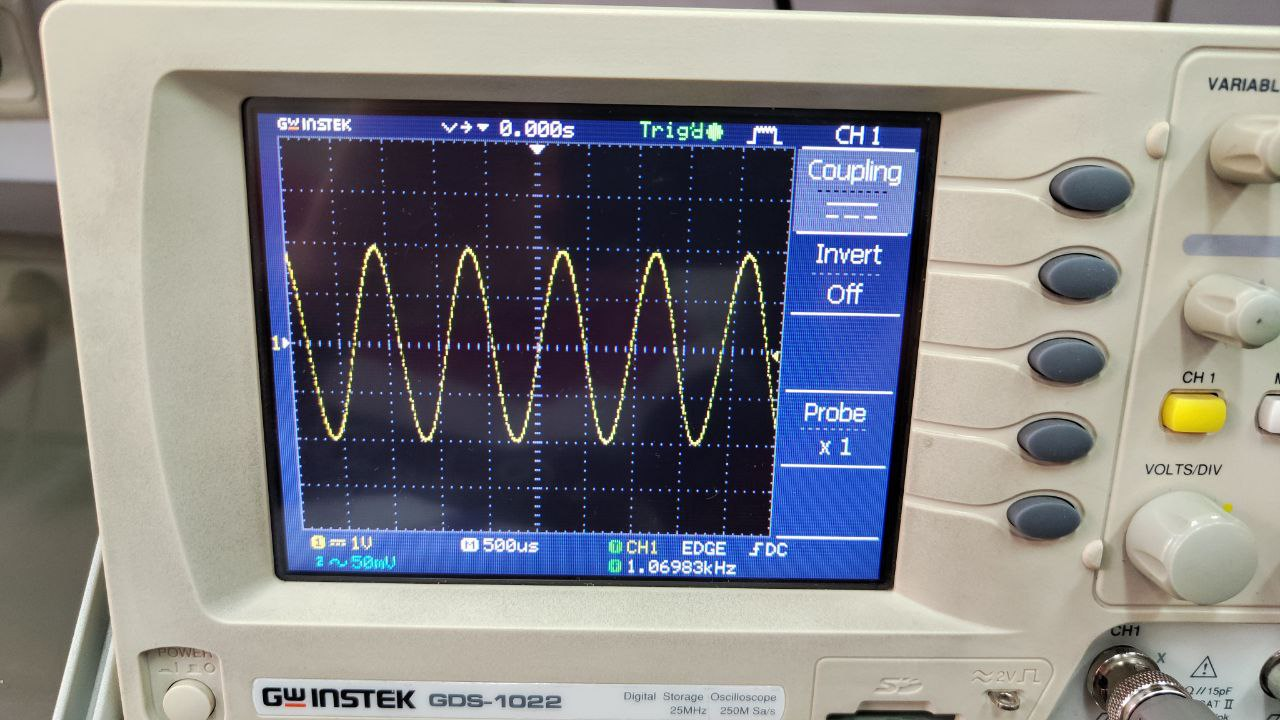
\includegraphics[scale=\PicScale]{Fig/1.jpeg}
            \caption{wave on oscilloscope.}
        \end{center}
    \end{figure}
}
\end{subquestion}

\begin{subquestion}{Investigate the impact of attenuation, offset, and duty knobs on the signal.}
\answer{
    \begin{figure}[H]
        \begin{center}
            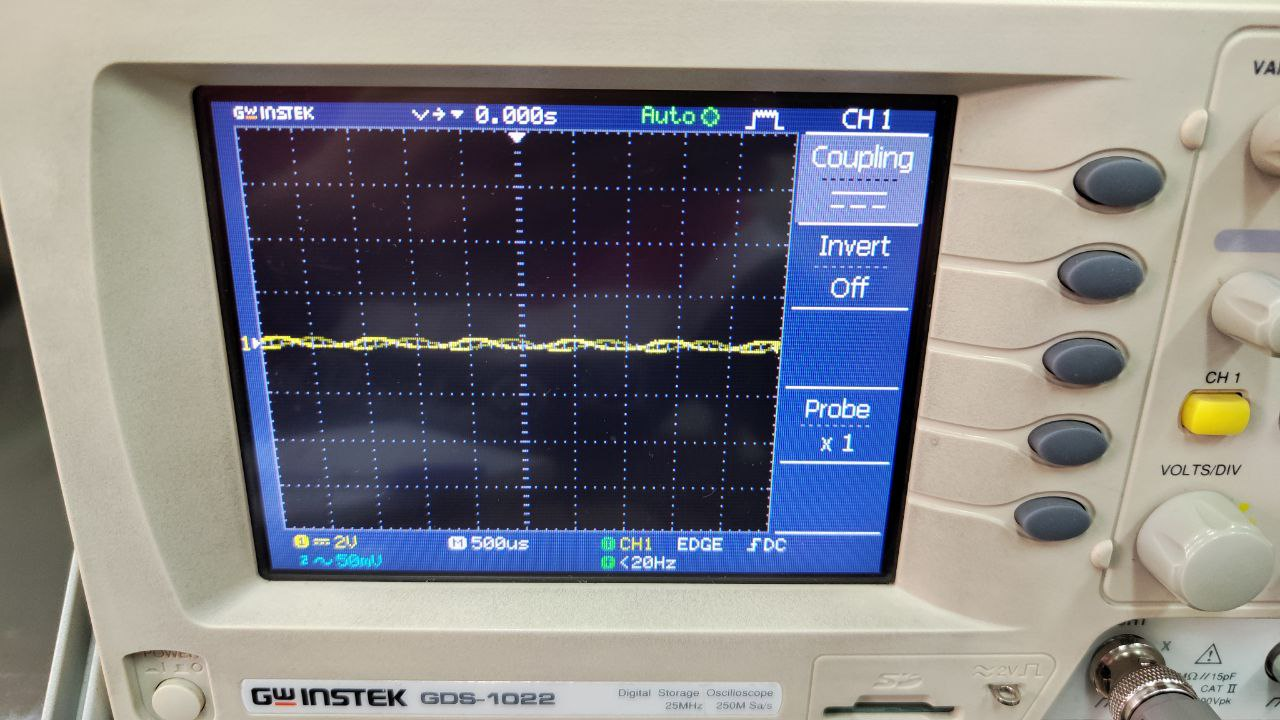
\includegraphics[scale=0.1]{Fig/2.jpeg}
            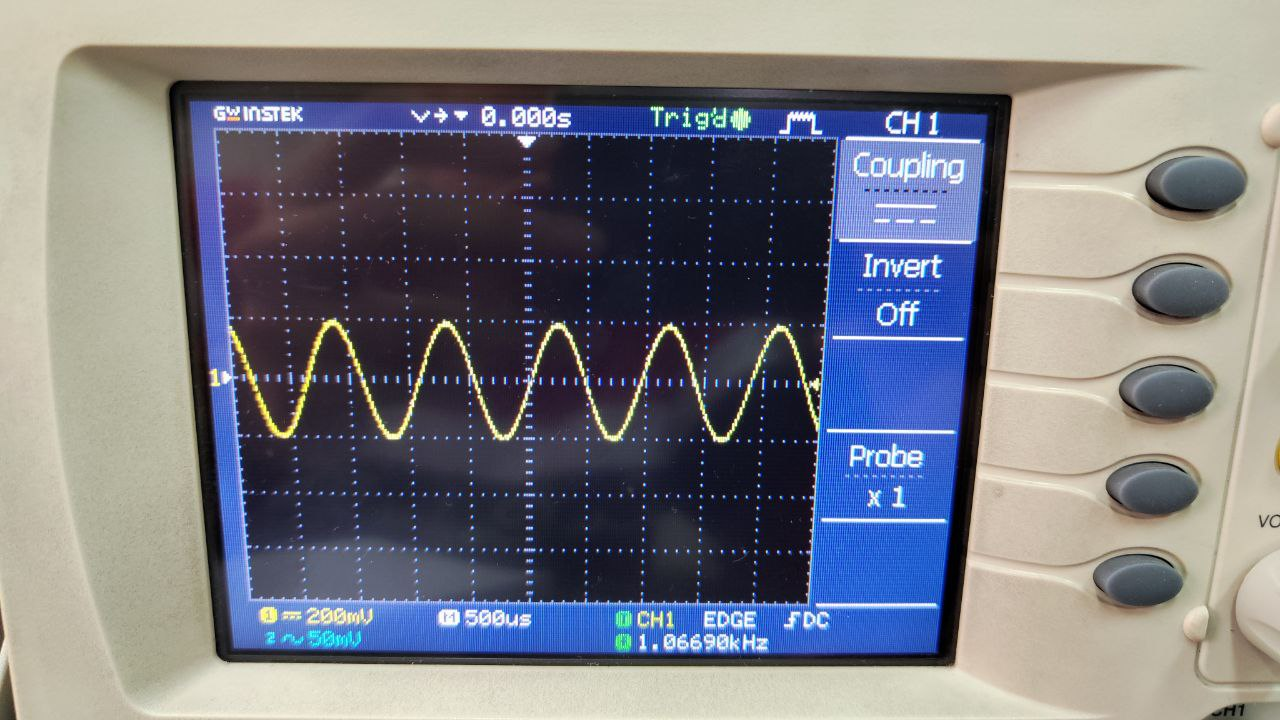
\includegraphics[scale=0.1]{Fig/3.jpeg}
            \caption{attenuation set.}
        \end{center}
    \end{figure}

    \begin{figure}[H]
        \begin{center}
            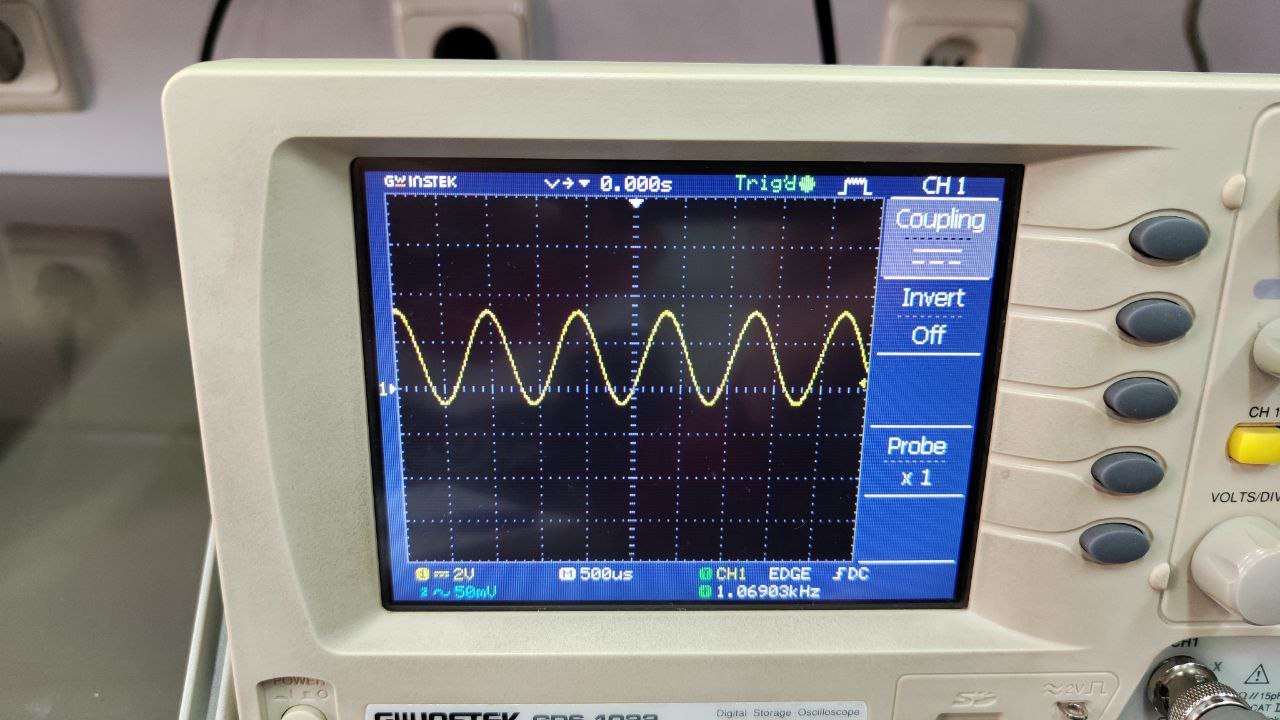
\includegraphics[scale=0.1]{Fig/4.jpeg}
            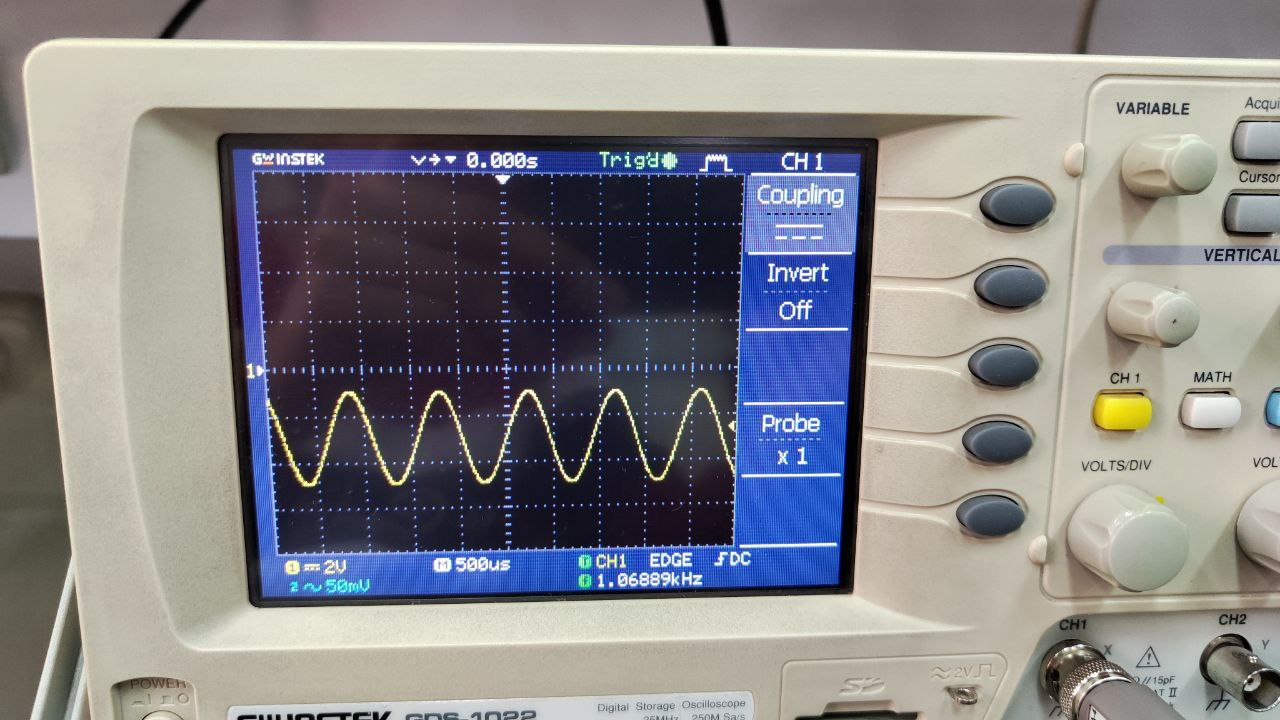
\includegraphics[scale=0.1]{Fig/5.jpeg}
            \caption{gave offset.}
        \end{center}
    \end{figure}

    \begin{figure}[H]
        \begin{center}
            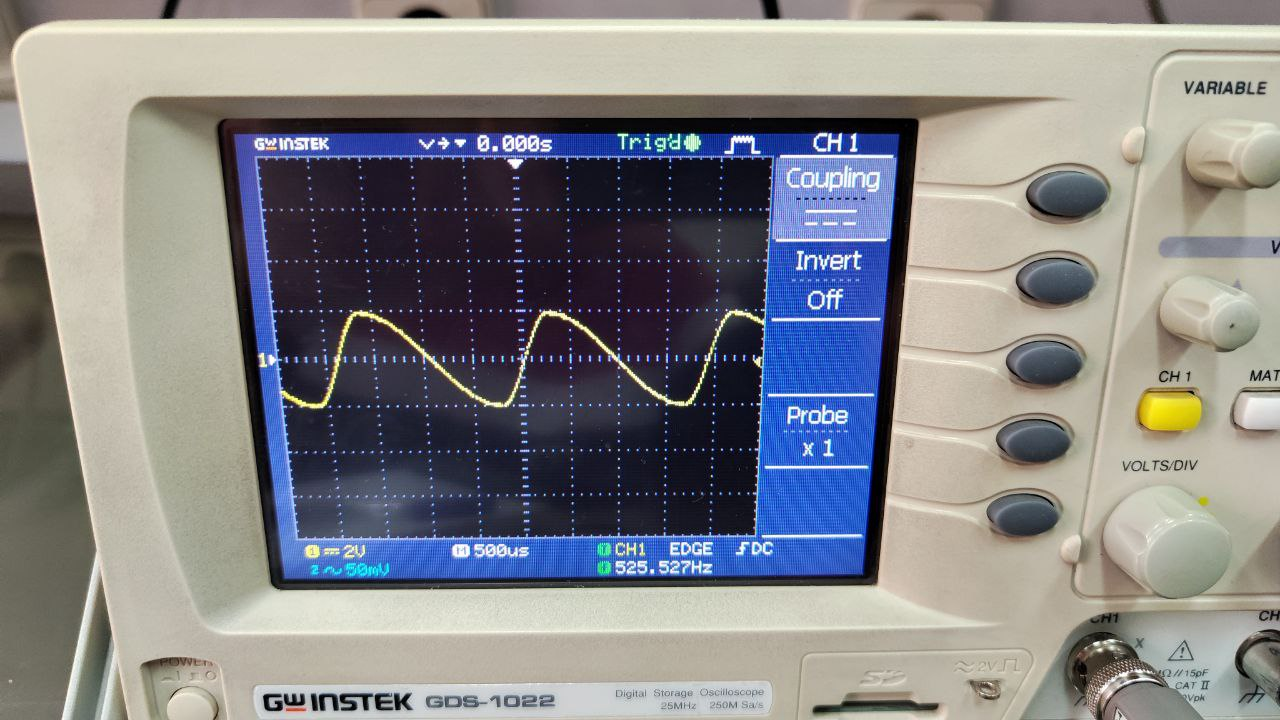
\includegraphics[scale=\PicScale]{Fig/6.jpeg}
            \caption{changed duty cycle.}
        \end{center}
    \end{figure}
}
\end{subquestion}

\begin{subquestion}{Repeat this part for triangle and square waves.}
\answer{
    \begin{figure}[H]
        \begin{center}
            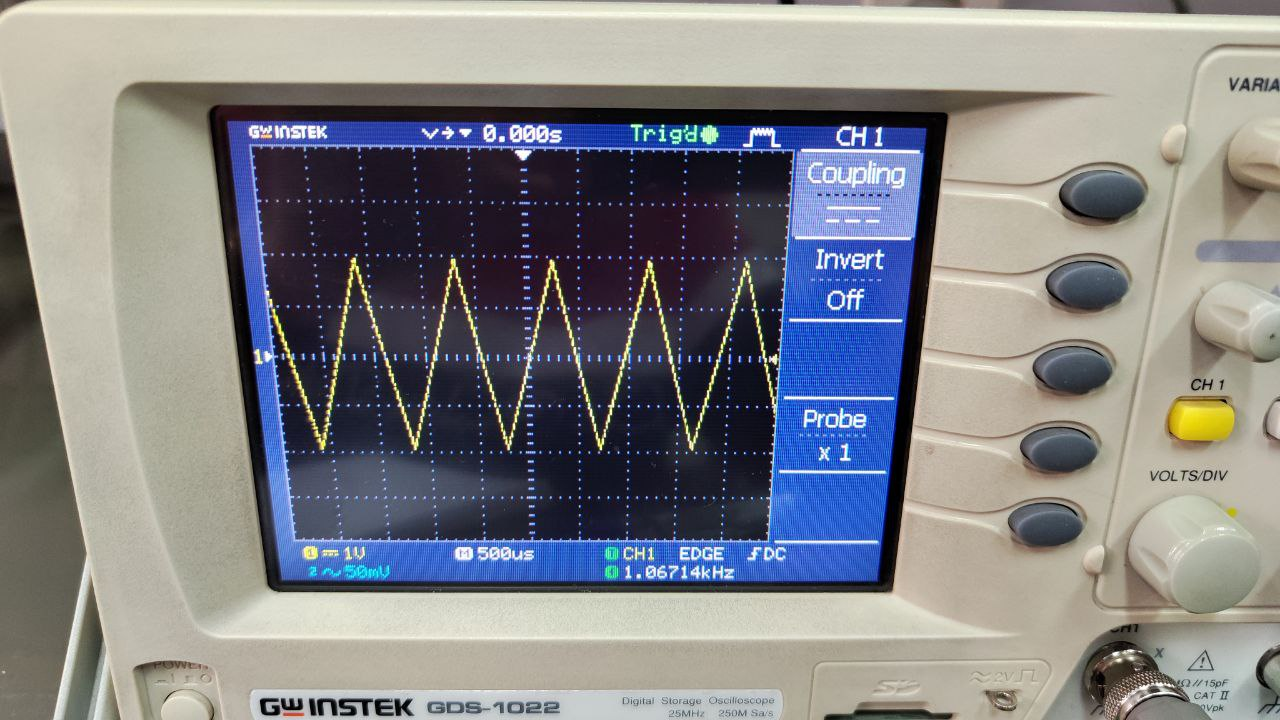
\includegraphics[scale=\PicScale]{Fig/7.jpeg}
            \caption{triangle wave base form.}
        \end{center}
    \end{figure}

    \begin{figure}[H]
        \begin{center}
            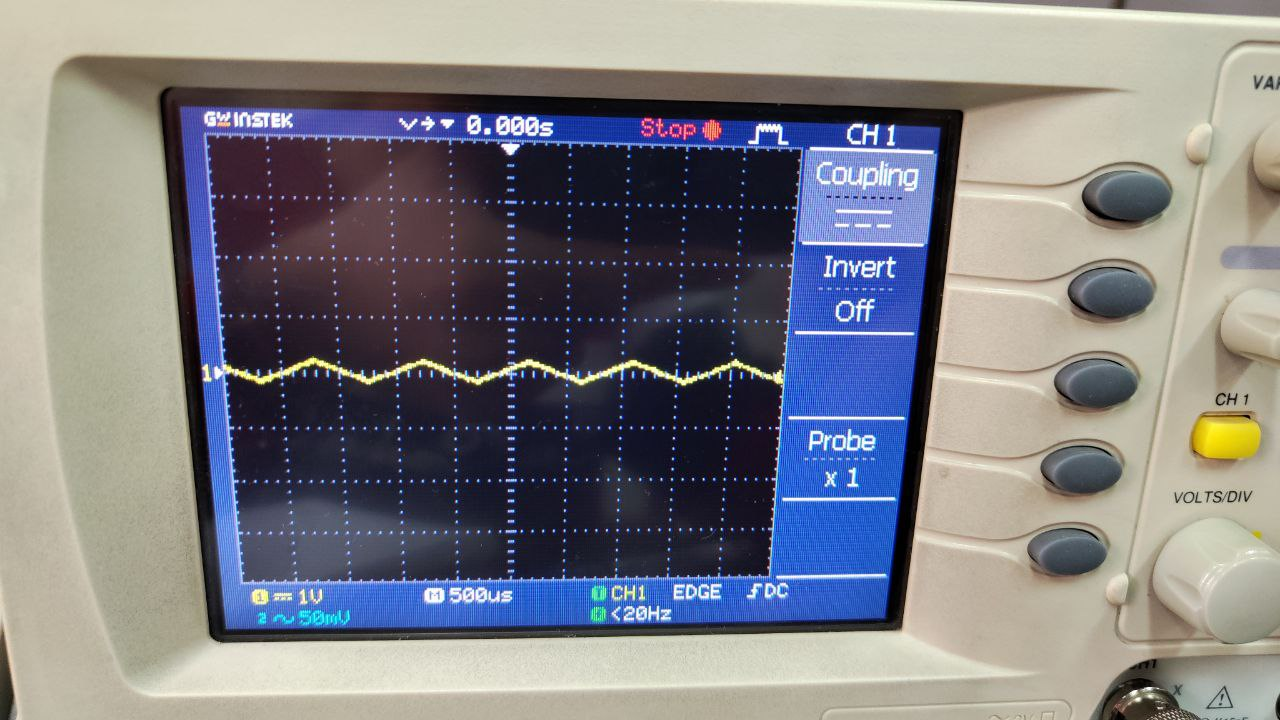
\includegraphics[scale=0.1]{Fig/8.jpeg}
            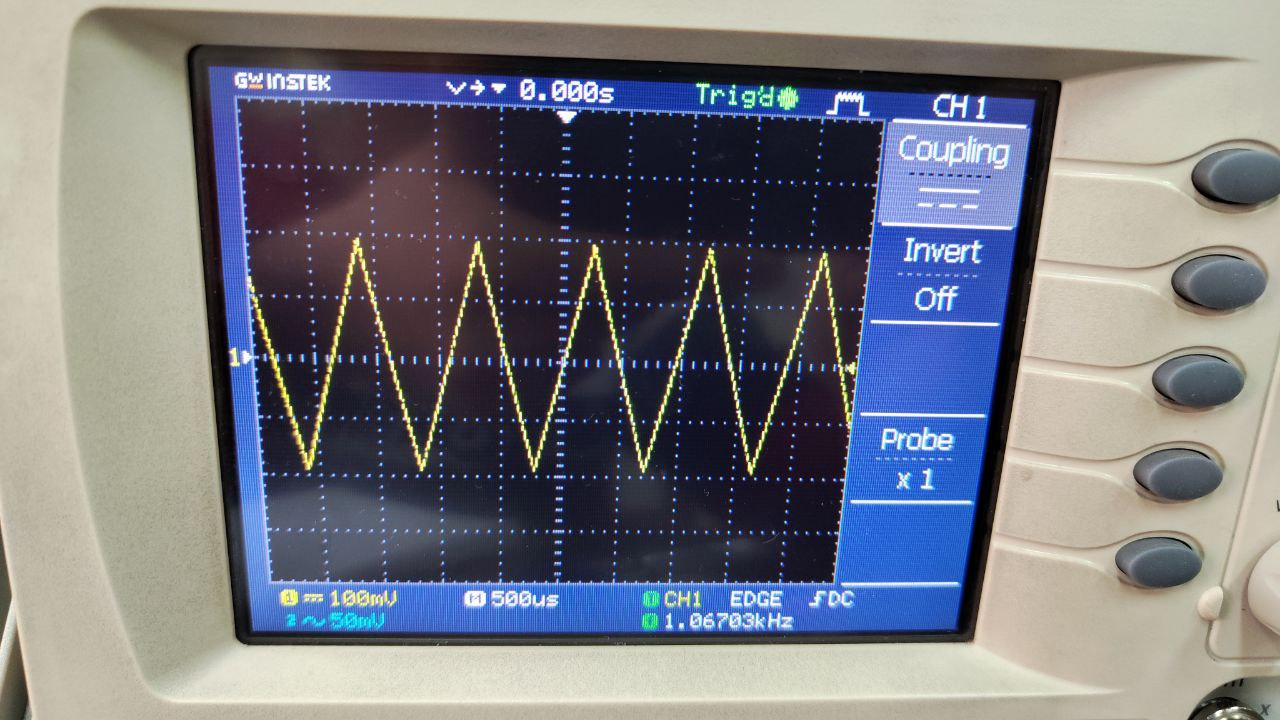
\includegraphics[scale=0.1]{Fig/9.jpeg}
            \caption{attenuation set.}
        \end{center}
    \end{figure}

    \begin{figure}[H]
        \begin{center}
            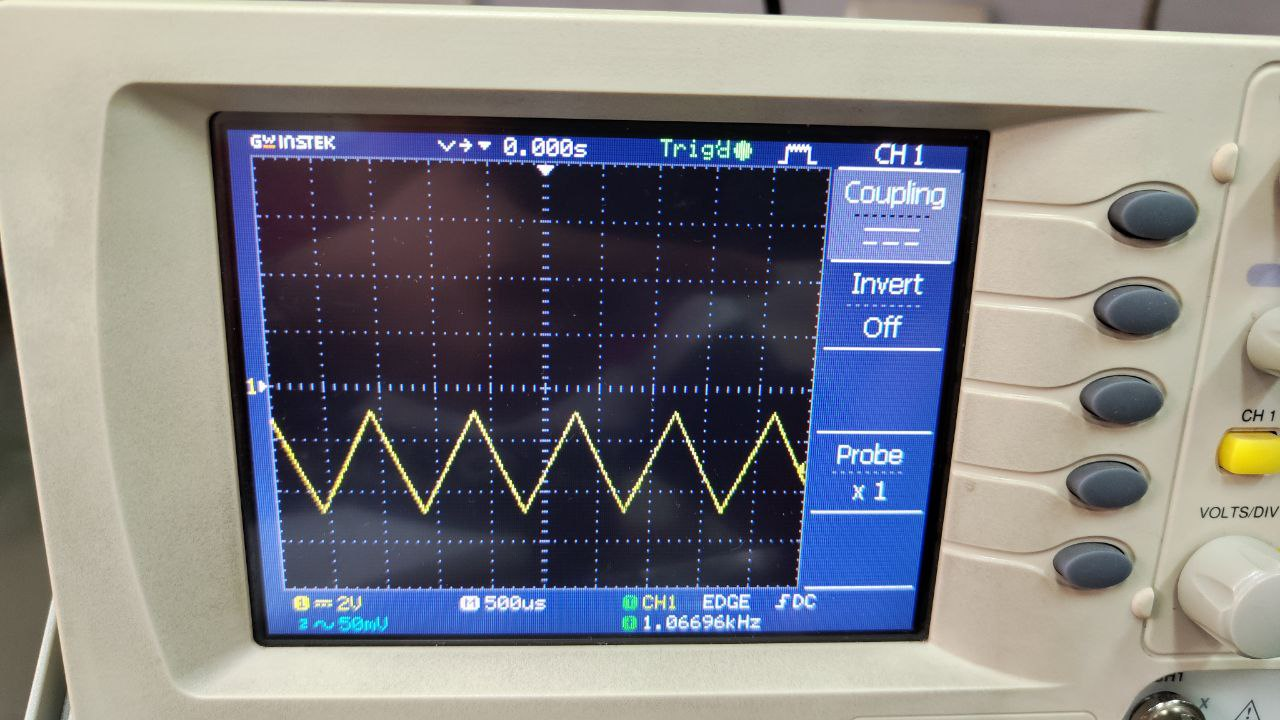
\includegraphics[scale=0.1]{Fig/10.jpeg}
            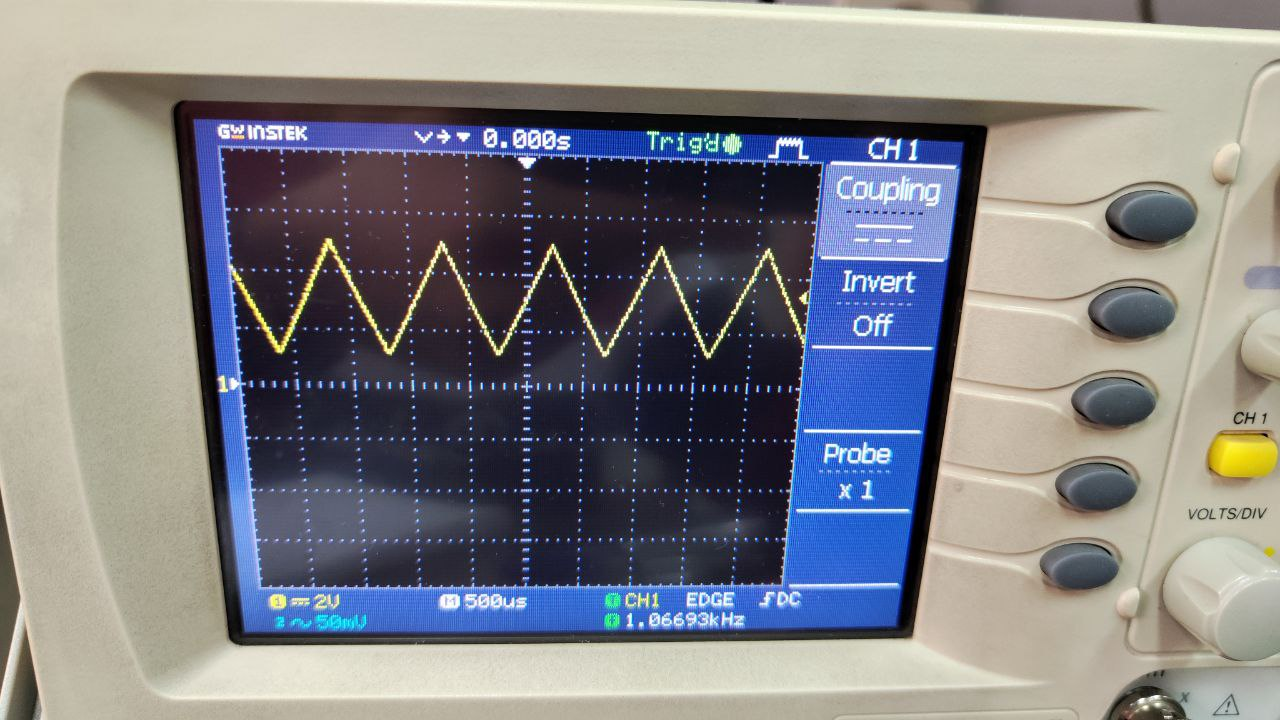
\includegraphics[scale=0.1]{Fig/11.jpeg}
            \caption{gave offset.}
        \end{center}
    \end{figure}

    \begin{figure}[H]
        \begin{center}
            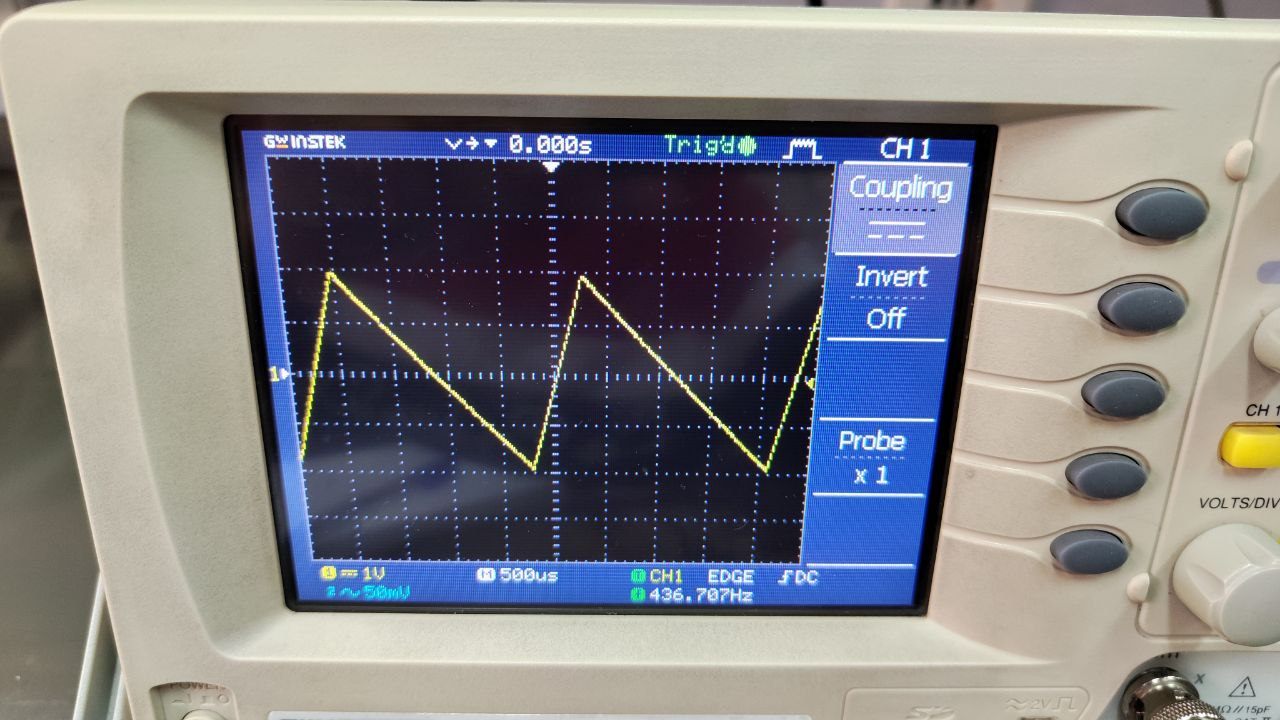
\includegraphics[scale=\PicScale]{Fig/12.jpeg}
            \caption{changed duty cycle.}
        \end{center}
    \end{figure}

    \begin{figure}[H]
        \begin{center}
            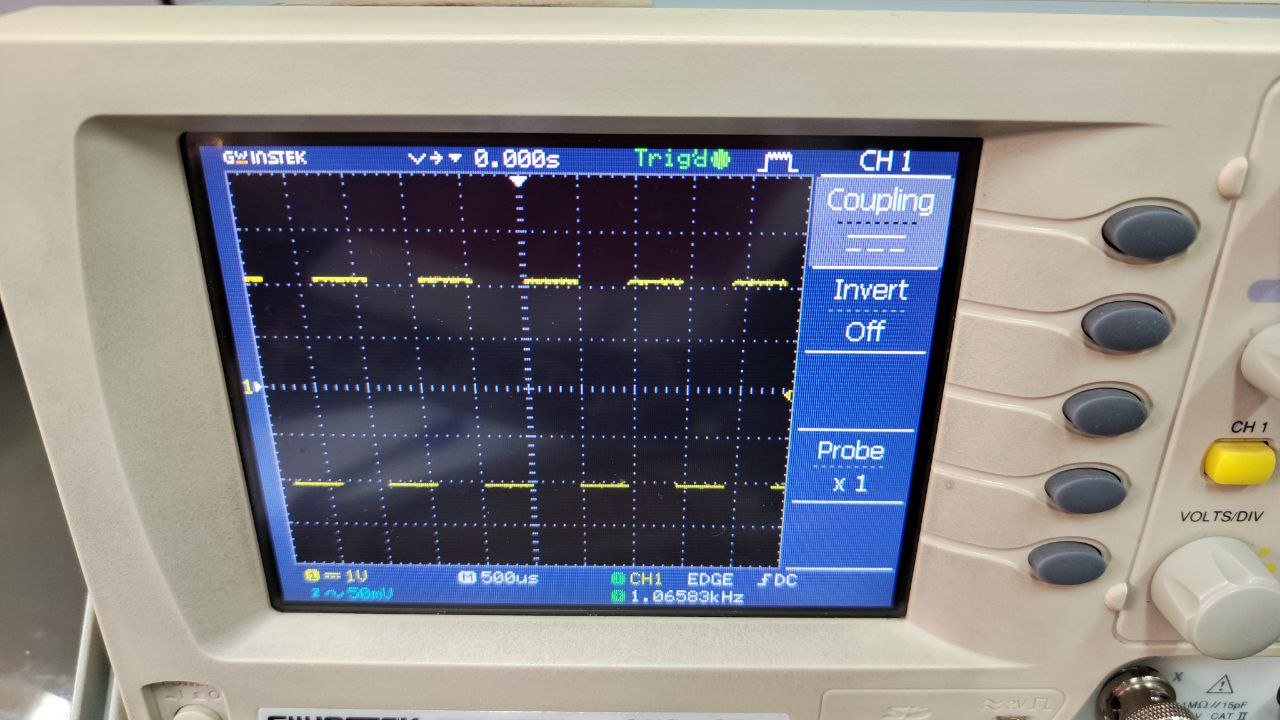
\includegraphics[scale=\PicScale]{Fig/13.jpeg}
            \caption{square wave base form.}
        \end{center}
    \end{figure}

    \begin{figure}[H]
        \begin{center}
            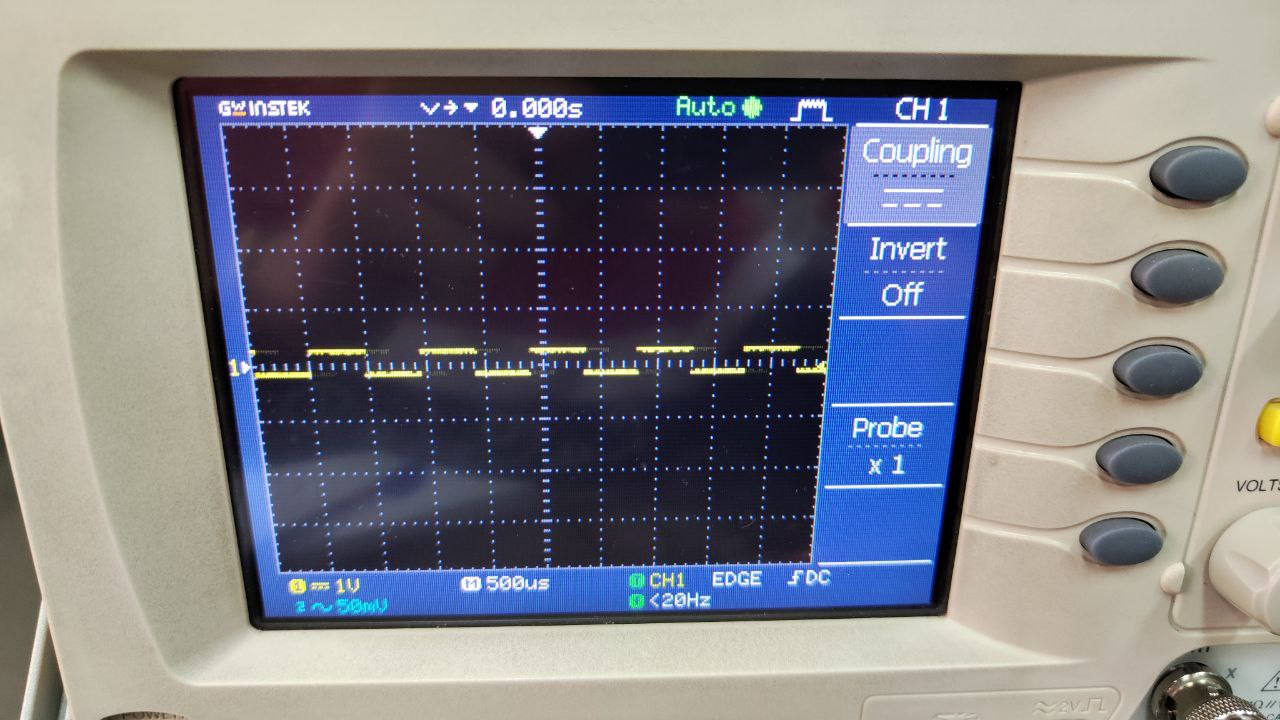
\includegraphics[scale=0.1]{Fig/14.jpeg}
            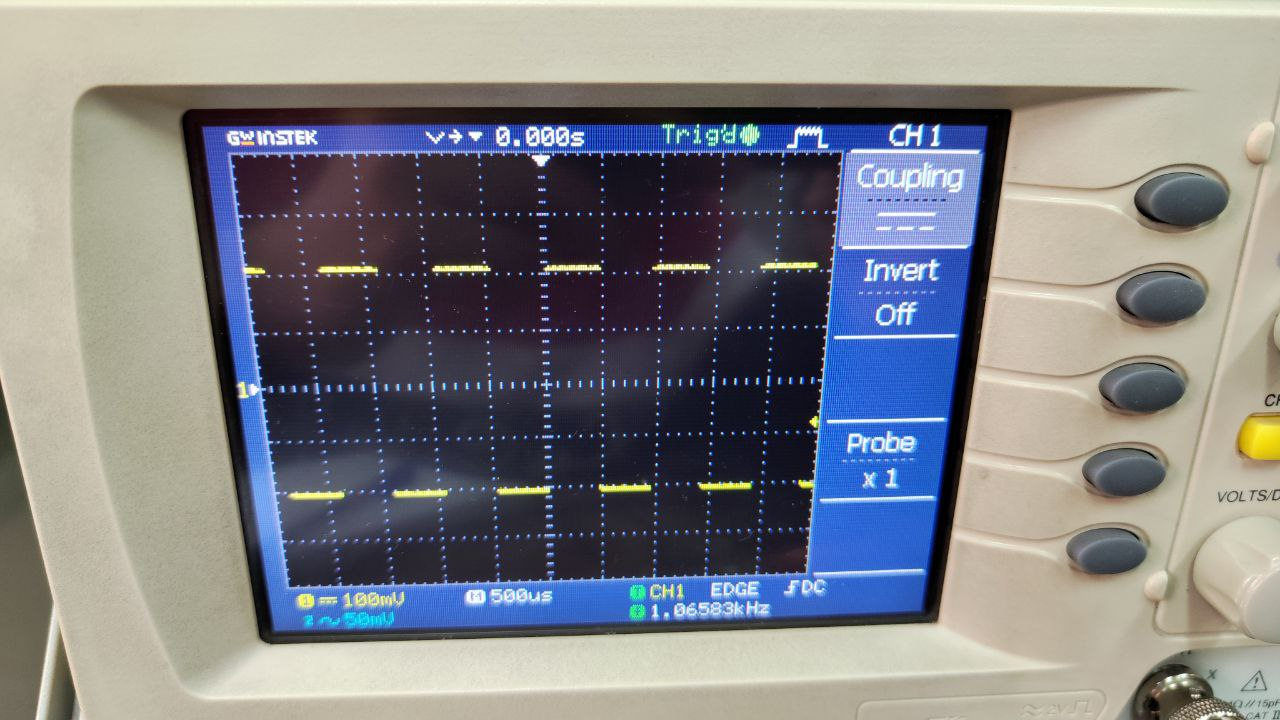
\includegraphics[scale=0.1]{Fig/15.jpeg}
            \caption{attenuation set.}
        \end{center}
    \end{figure}

    \begin{figure}[H]
        \begin{center}
            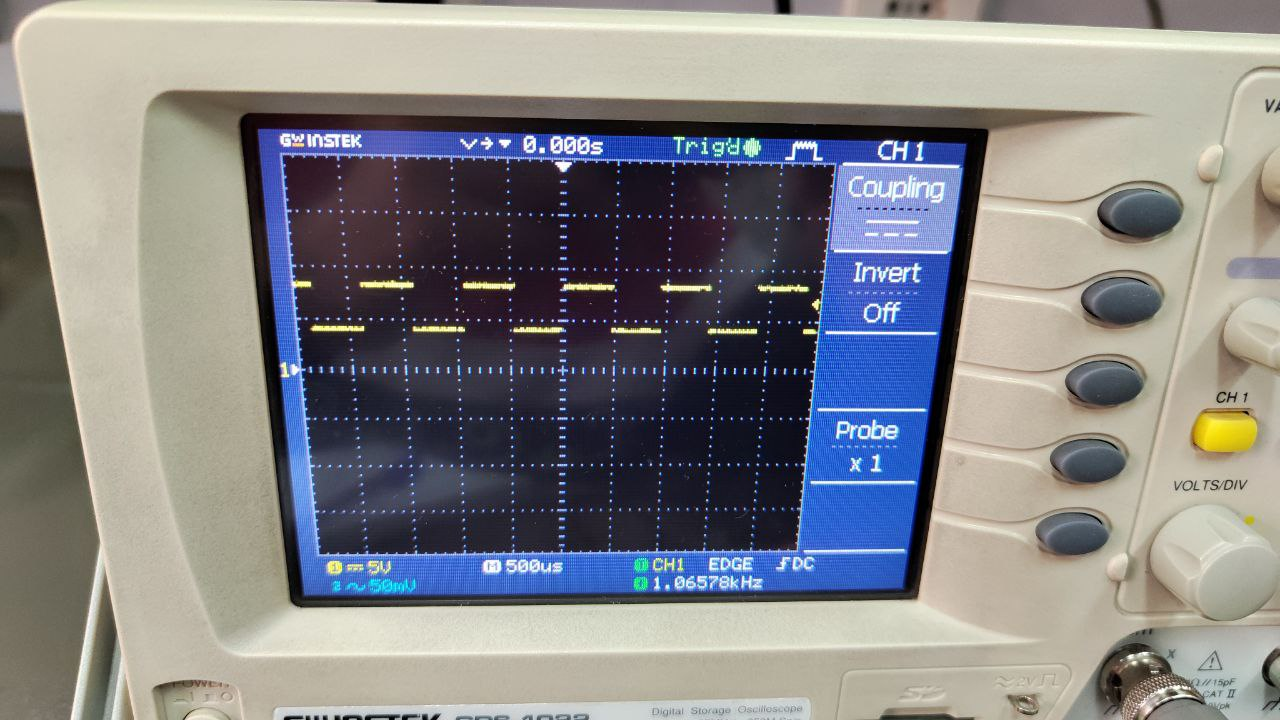
\includegraphics[scale=0.1]{Fig/16.jpeg}
            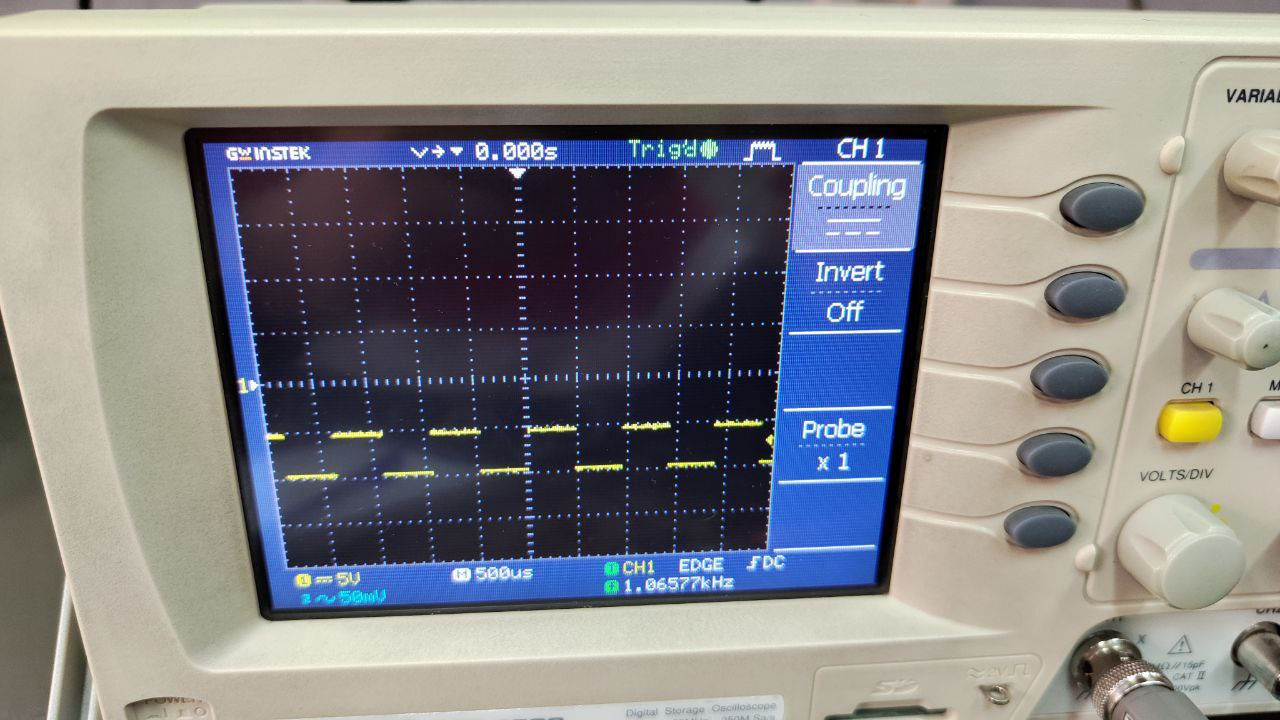
\includegraphics[scale=0.1]{Fig/17.jpeg}
            \caption{gave offset.}
        \end{center}
    \end{figure}

    \begin{figure}[H]
        \begin{center}
            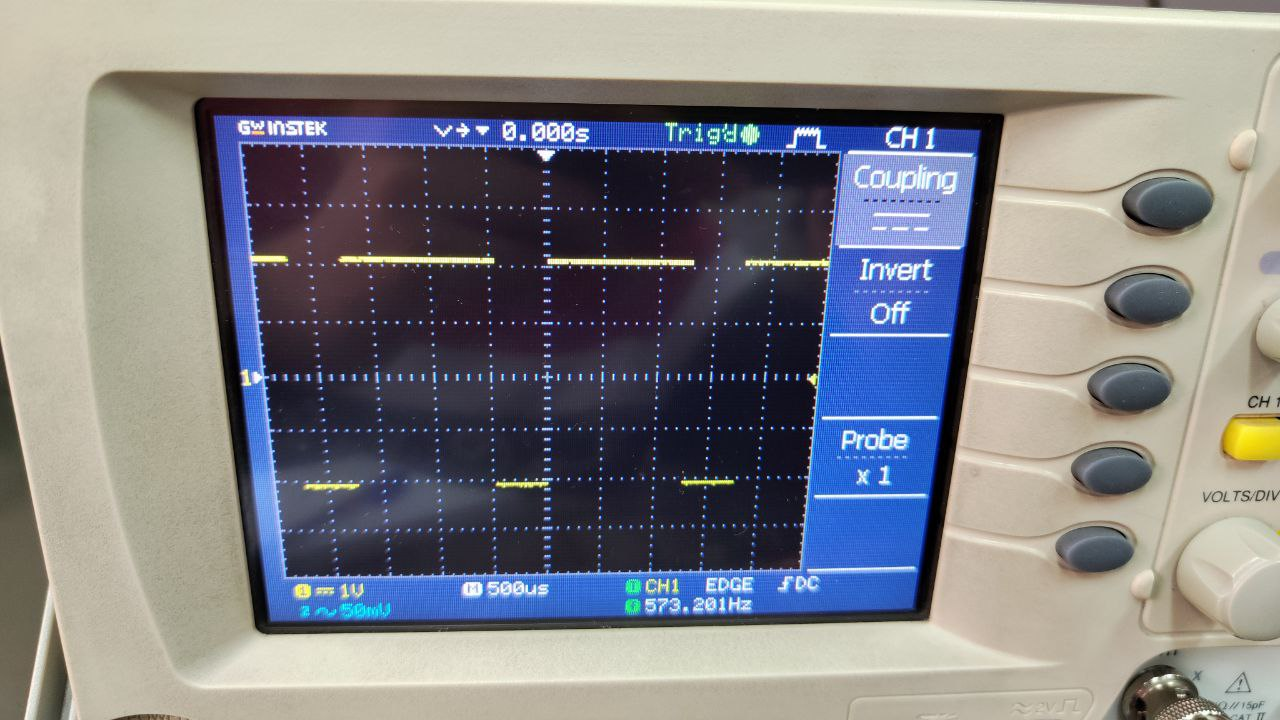
\includegraphics[scale=\PicScale]{Fig/18.jpeg}
            \caption{changed duty cycle.}
        \end{center}
    \end{figure}
}
\end{subquestion}

\end{question}

%----------------------------------------------------------------------------------------
%	QUESTION 2
%----------------------------------------------------------------------------------------

\begin{question}

\questiontext{Set the controls of the function generator to produce a sine wave of $50$ Hz frequency and $1$ V amplitude around an offset of $1$ V.}

\begin{subquestion}{Use the oscilloscope to see the wave and read its frequency and amplitude.}
\answer{
    \begin{figure}[H]
        \begin{center}
            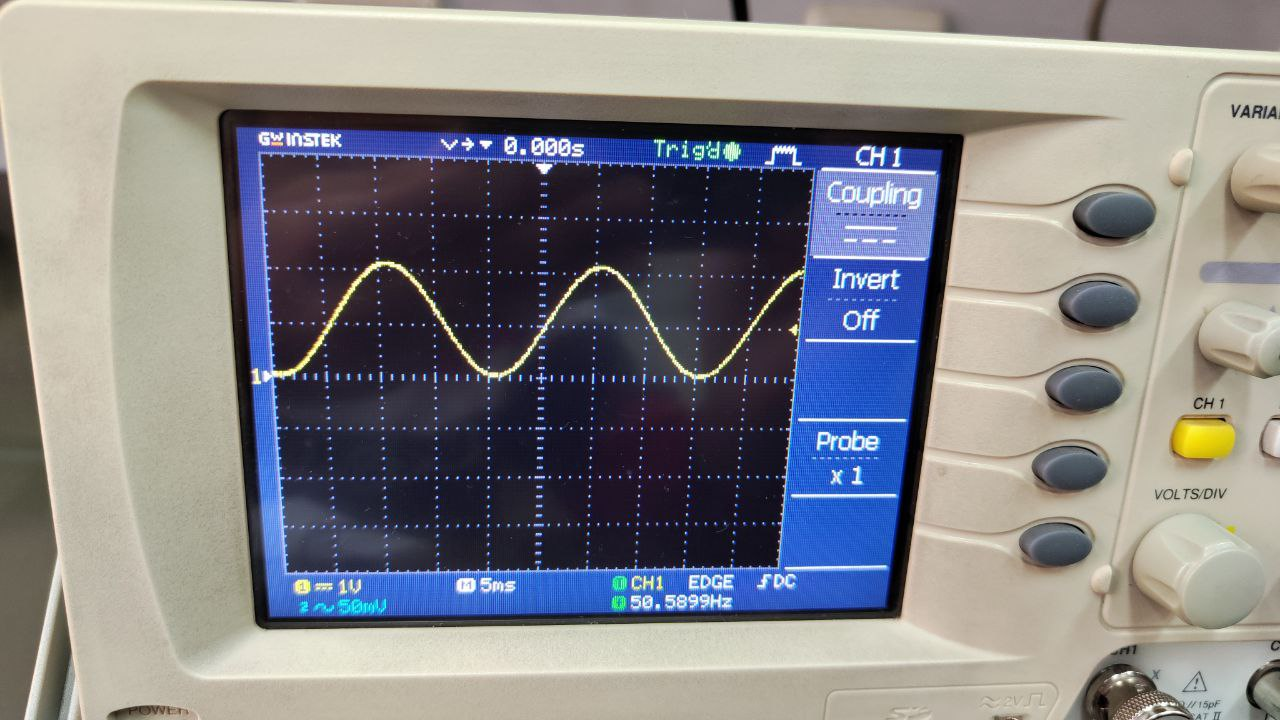
\includegraphics[scale=\PicScale]{Fig/19.jpeg}
            \caption{triangle wave base form.}
        \end{center}
    \end{figure}
}
\end{subquestion}

\begin{subquestion}{Measure the voltage of the wave using a multi-meter in AC and DC modes. Compare the readings with that of the oscilloscope and interpret the results.}
\answer{
    \begin{figure}[H]
        \begin{center}
            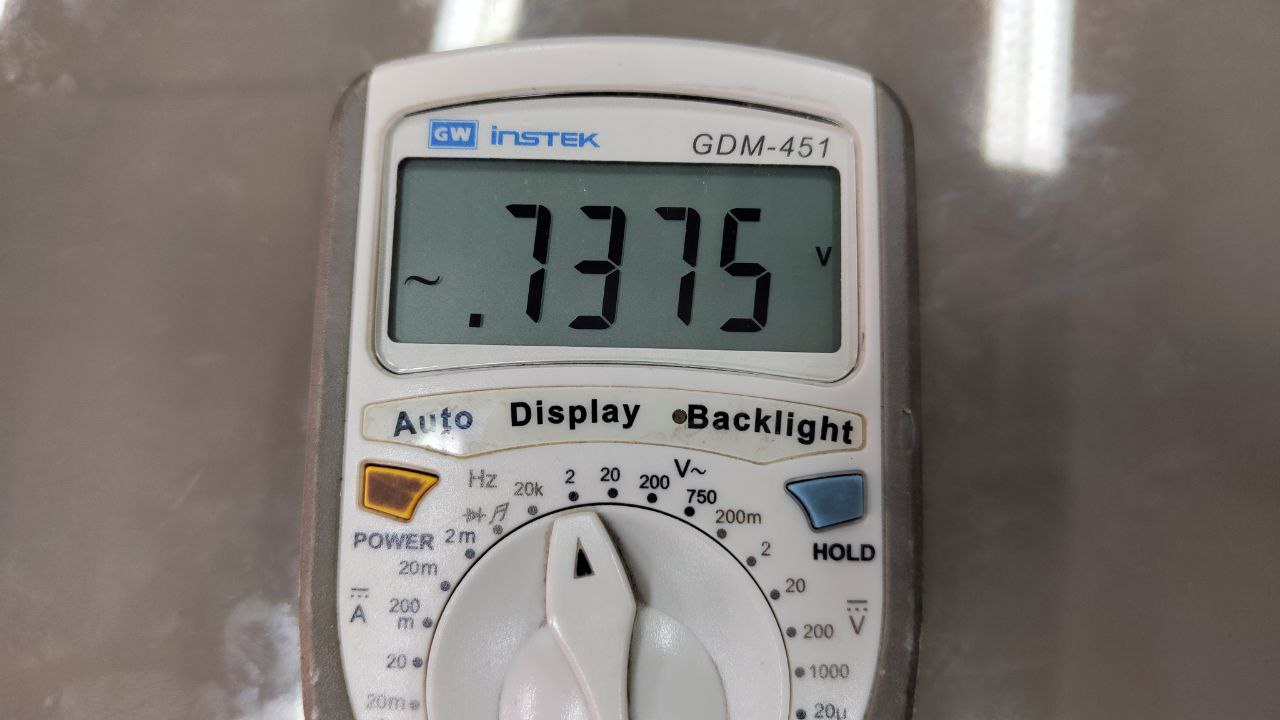
\includegraphics[scale=\PicScale]{Fig/20.jpeg}
            \caption{$V_{AC}$.}
        \end{center}
    \end{figure}

    \begin{figure}[H]
        \begin{center}
            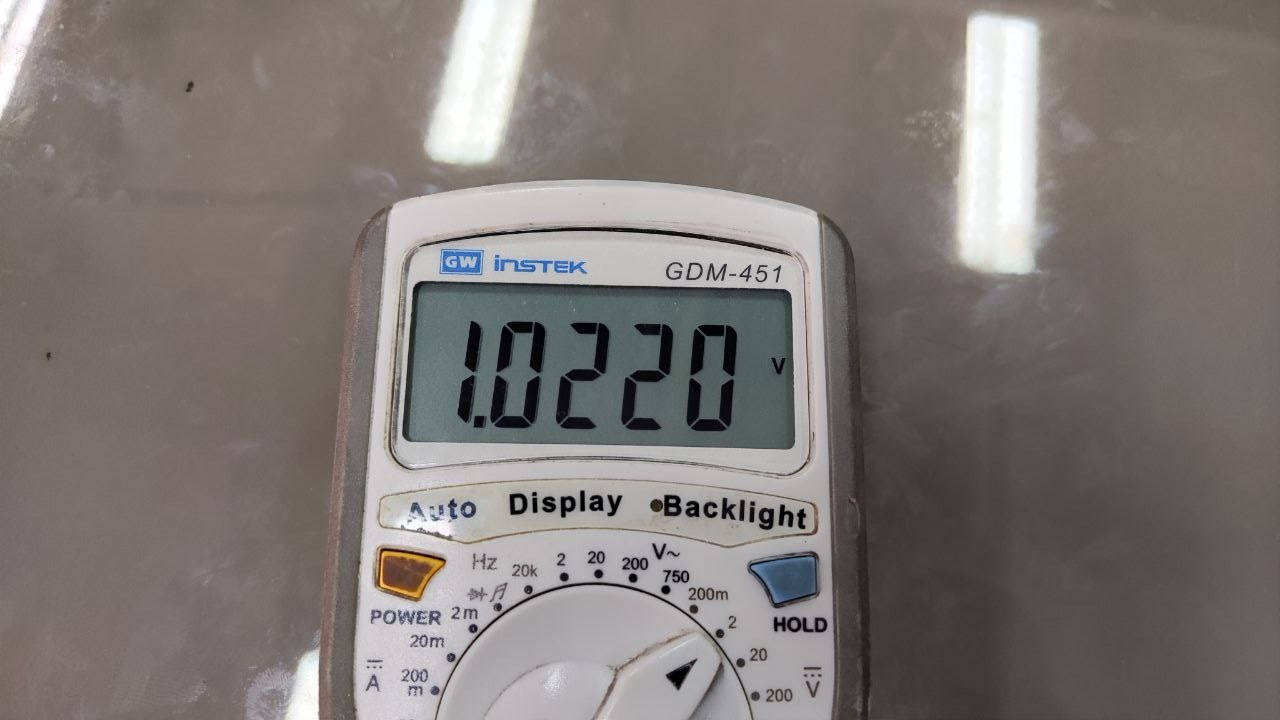
\includegraphics[scale=\PicScale]{Fig/21.jpeg}
            \caption{$V_{DC}$.}
        \end{center}
    \end{figure}
}
\end{subquestion}

\begin{subquestion}{Change the frequency, amplitude, and offset of the wave and check the readings of the multi-meter and oscilloscope.}
\answer{
    \begin{figure}[H]
        \begin{center}
            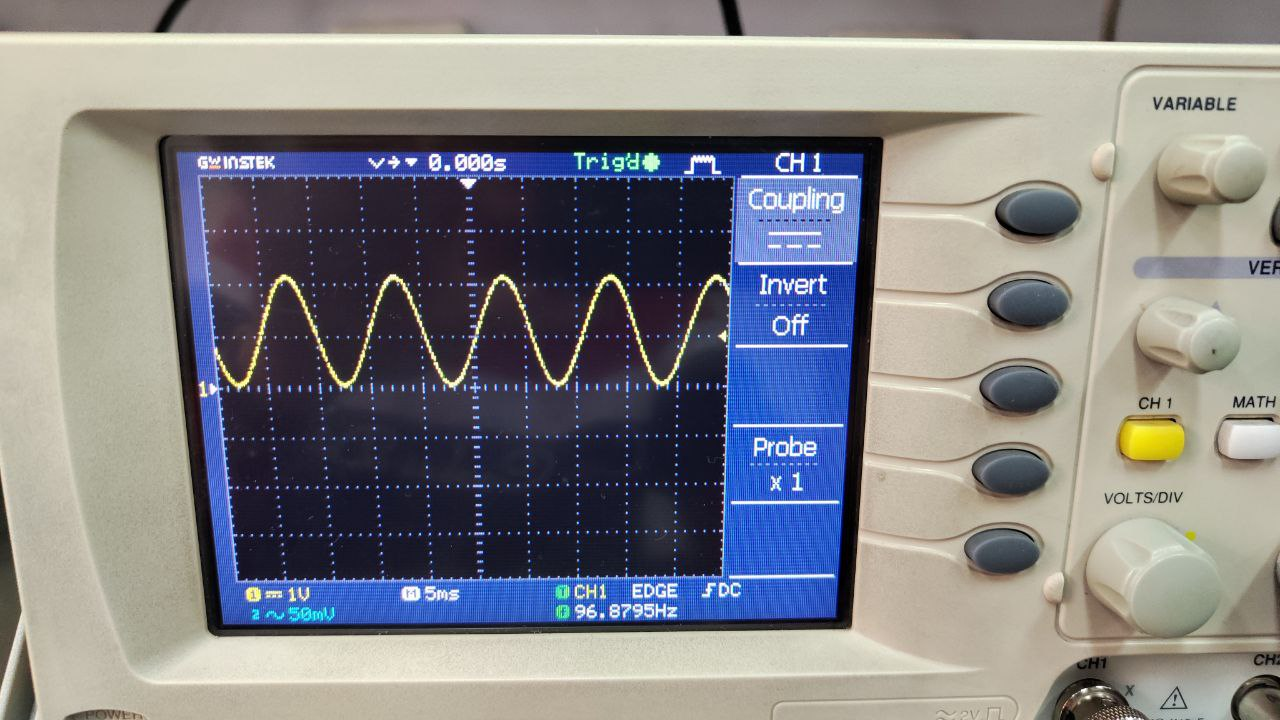
\includegraphics[scale=\PicScale]{Fig/22.jpeg}
            \caption{frequency increased.}
        \end{center}
    \end{figure}

    \begin{figure}[H]
        \begin{center}
            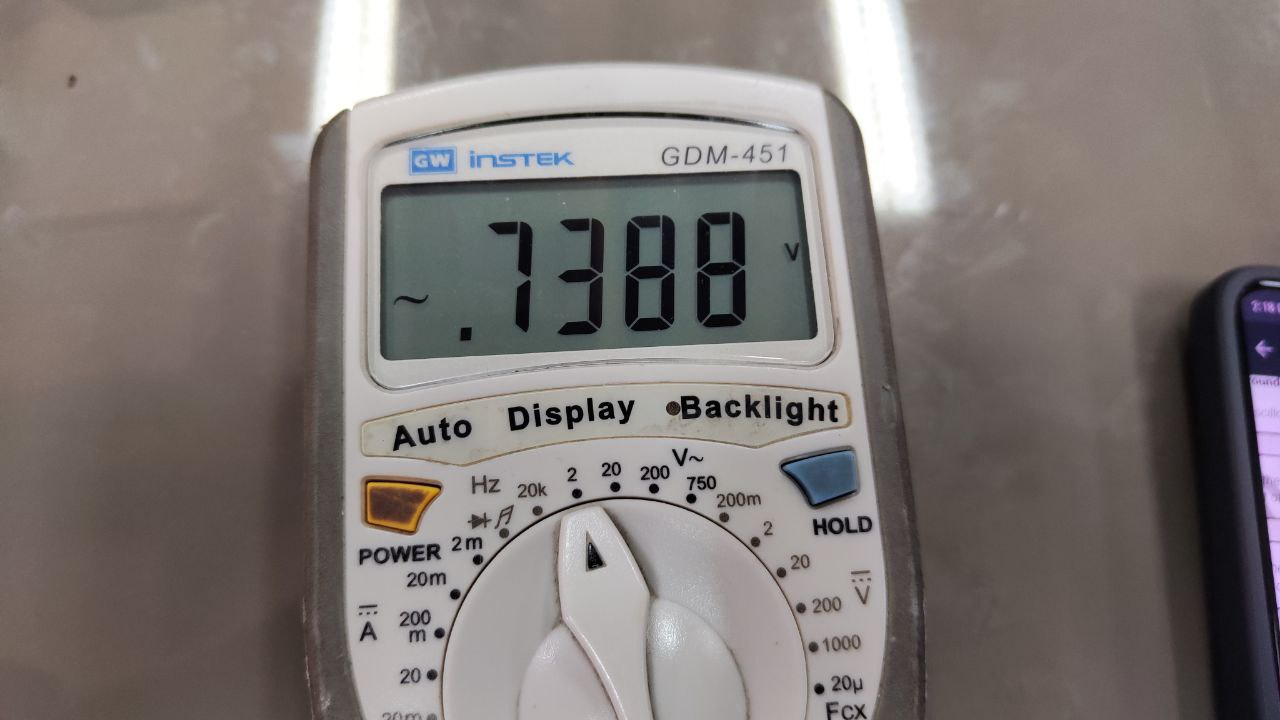
\includegraphics[scale=\PicScale]{Fig/23.jpeg}
            \caption{$V_{AC}$.}
        \end{center}
    \end{figure}
    $V_{DC}$ didn't change.

    \begin{figure}[H]
        \begin{center}
            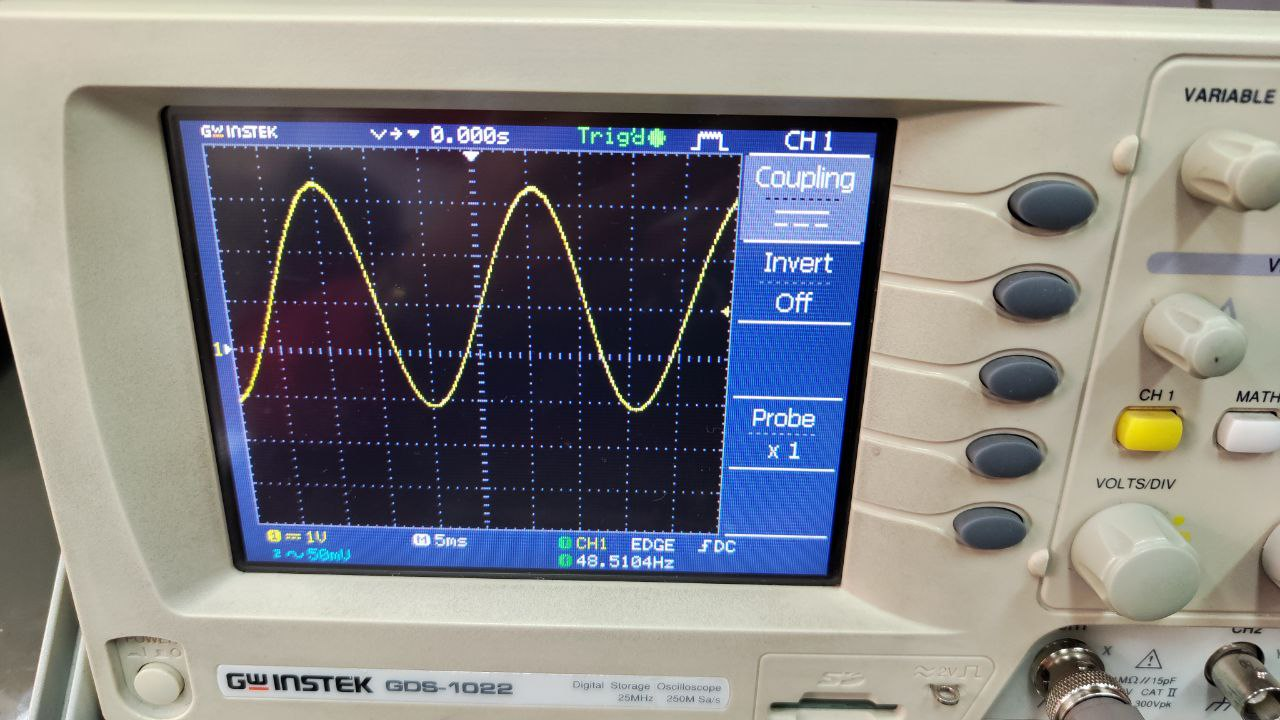
\includegraphics[scale=\PicScale]{Fig/24.jpeg}
            \caption{amplitude changed.}
        \end{center}
    \end{figure}
    \begin{figure}[H]
        \begin{center}
            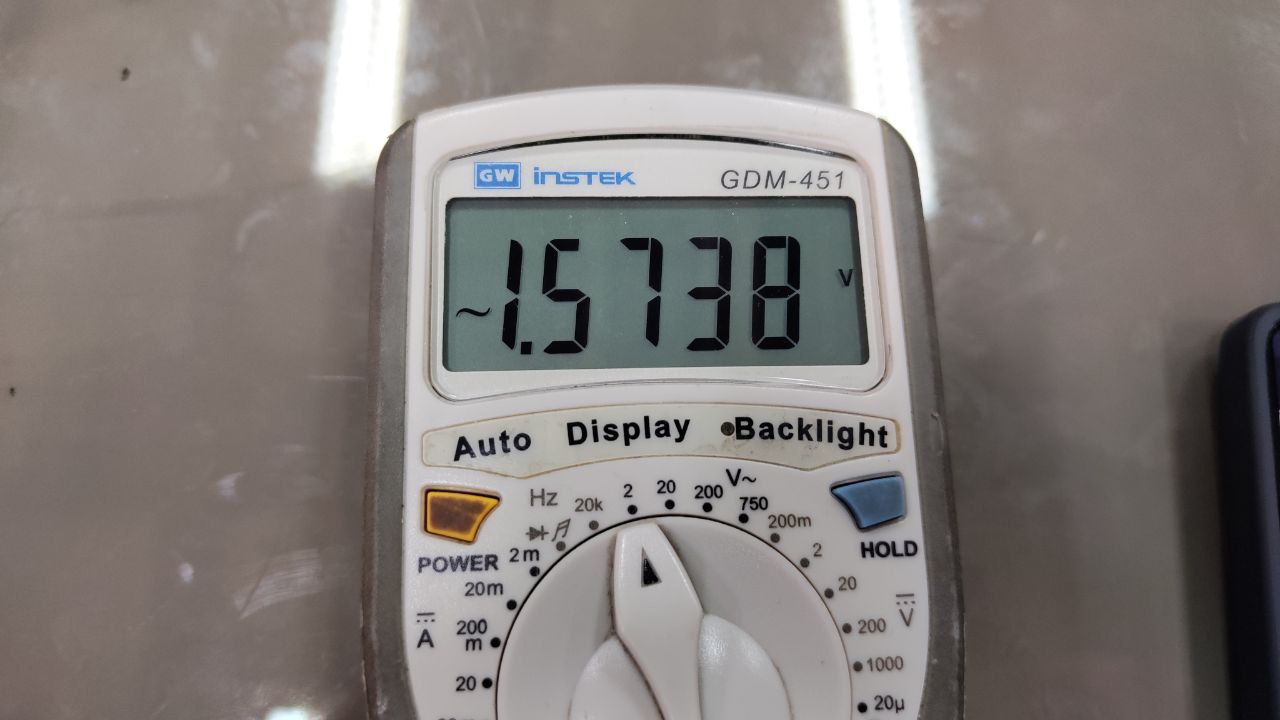
\includegraphics[scale=\PicScale]{Fig/25.jpeg}
            \caption{$V_{AC}$.}
        \end{center}
    \end{figure}

    \begin{figure}[H]
        \begin{center}
            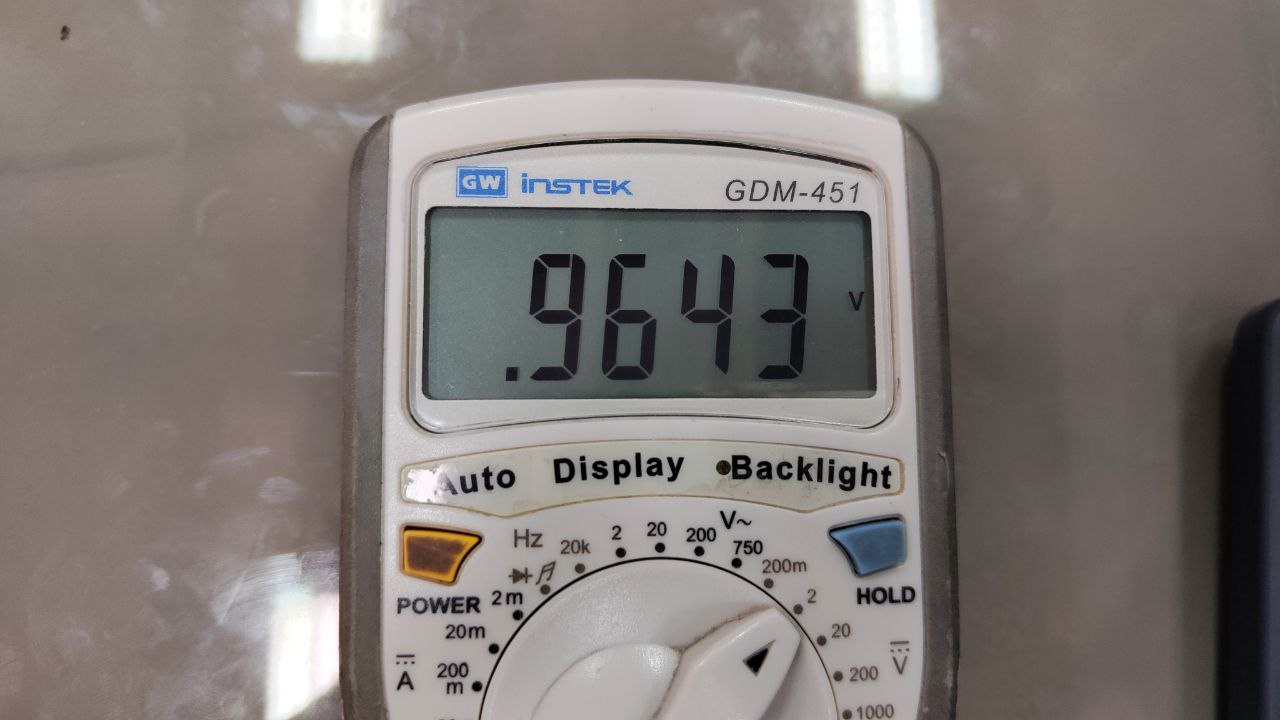
\includegraphics[scale=\PicScale]{Fig/26.jpeg}
            \caption{$V_{DC}$.}
        \end{center}
    \end{figure}

    \begin{figure}[H]
        \begin{center}
            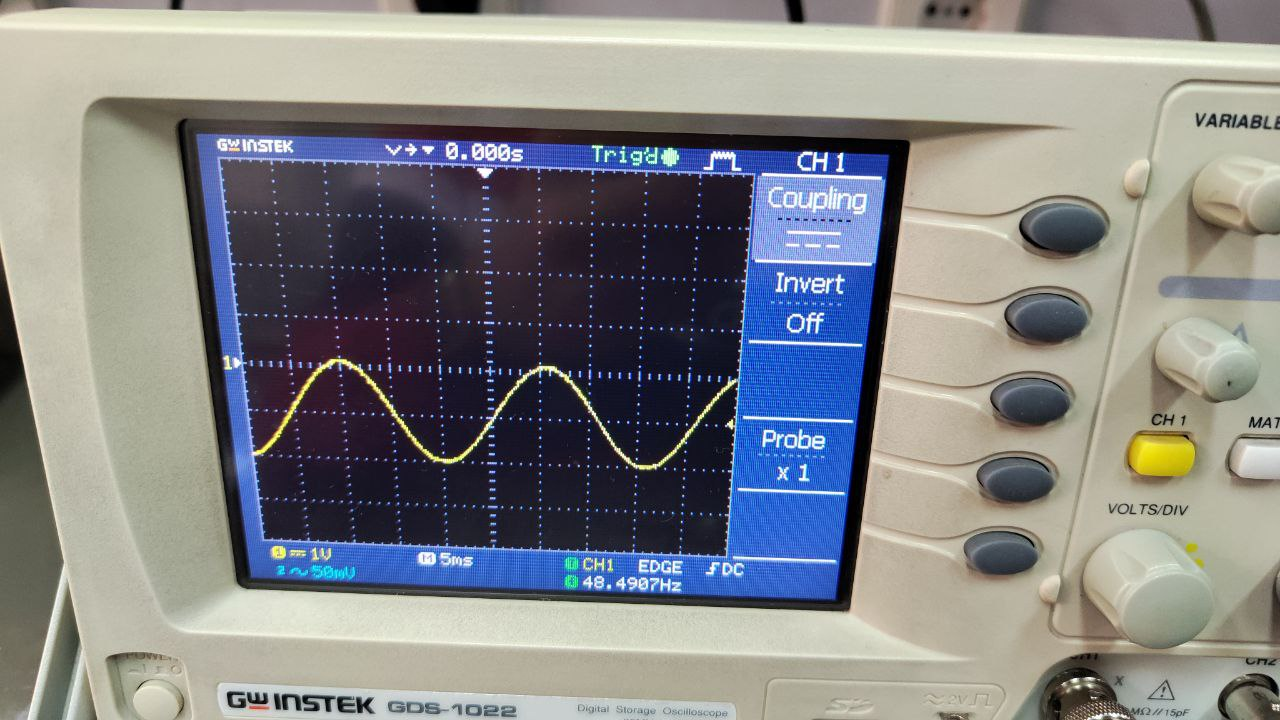
\includegraphics[scale=\PicScale]{Fig/27.jpeg}
            \caption{offset given.}
        \end{center}
    \end{figure}
    \begin{figure}[H]
        \begin{center}
            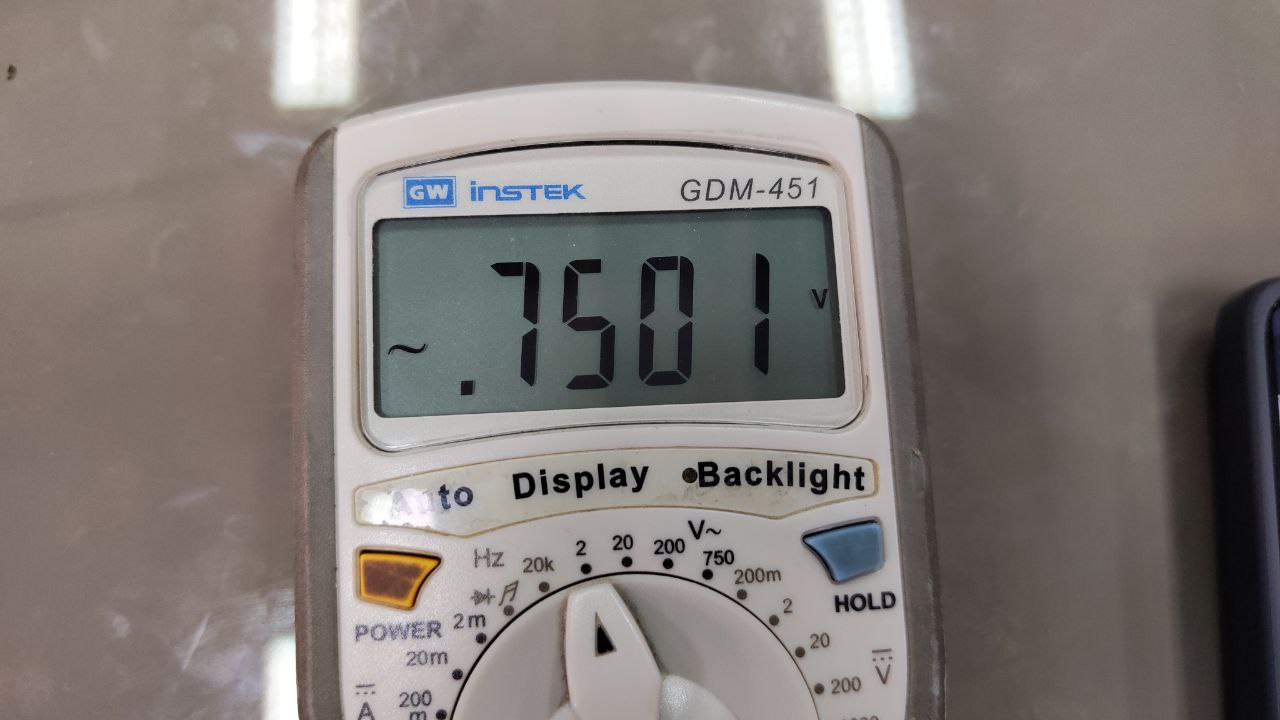
\includegraphics[scale=\PicScale]{Fig/28.jpeg}
            \caption{$V_{AC}$.}
        \end{center}
    \end{figure}

    \begin{figure}[H]
        \begin{center}
            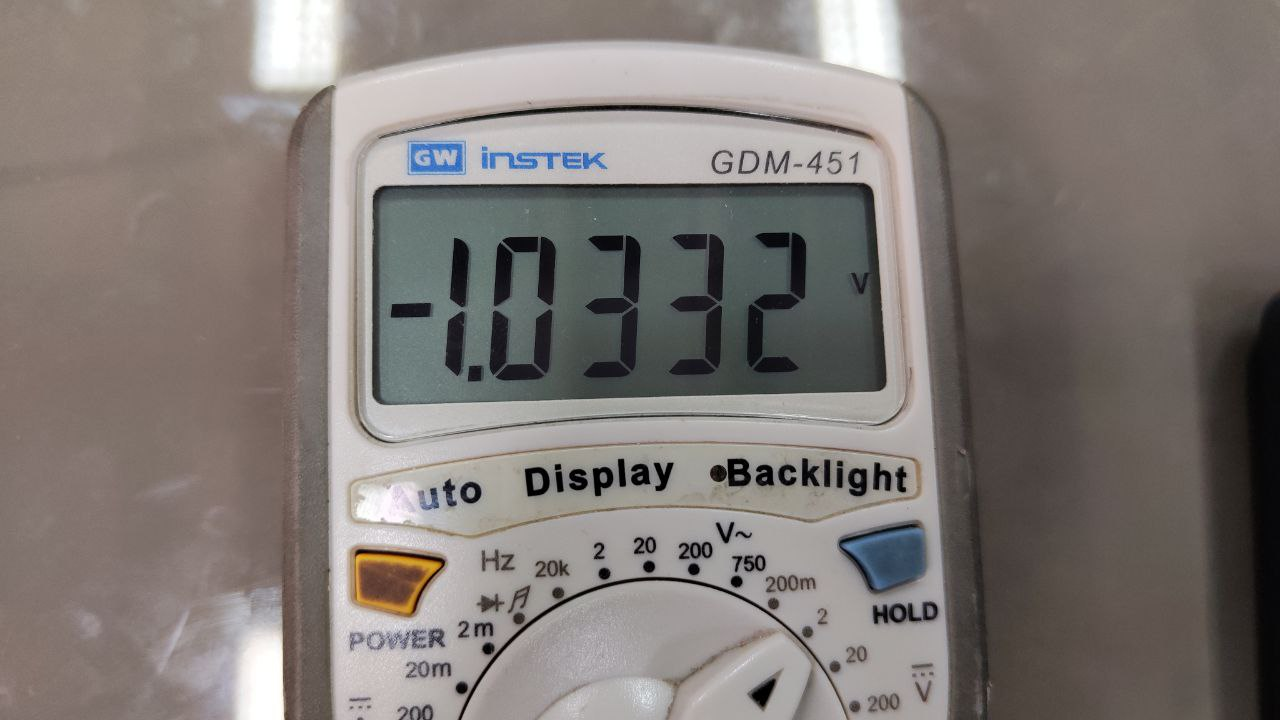
\includegraphics[scale=\PicScale]{Fig/29.jpeg}
            \caption{$V_{DC}$.}
        \end{center}
    \end{figure}
}
\end{subquestion}

\begin{subquestion}{Repeat this part for a square wave of $50\%$ duty cycle with a same frequency, amplitude, and offset as the previous sine wave. Investigate the readings as the duty cycle changes.}
\answer{
    \begin{figure}[H]
        \begin{center}
            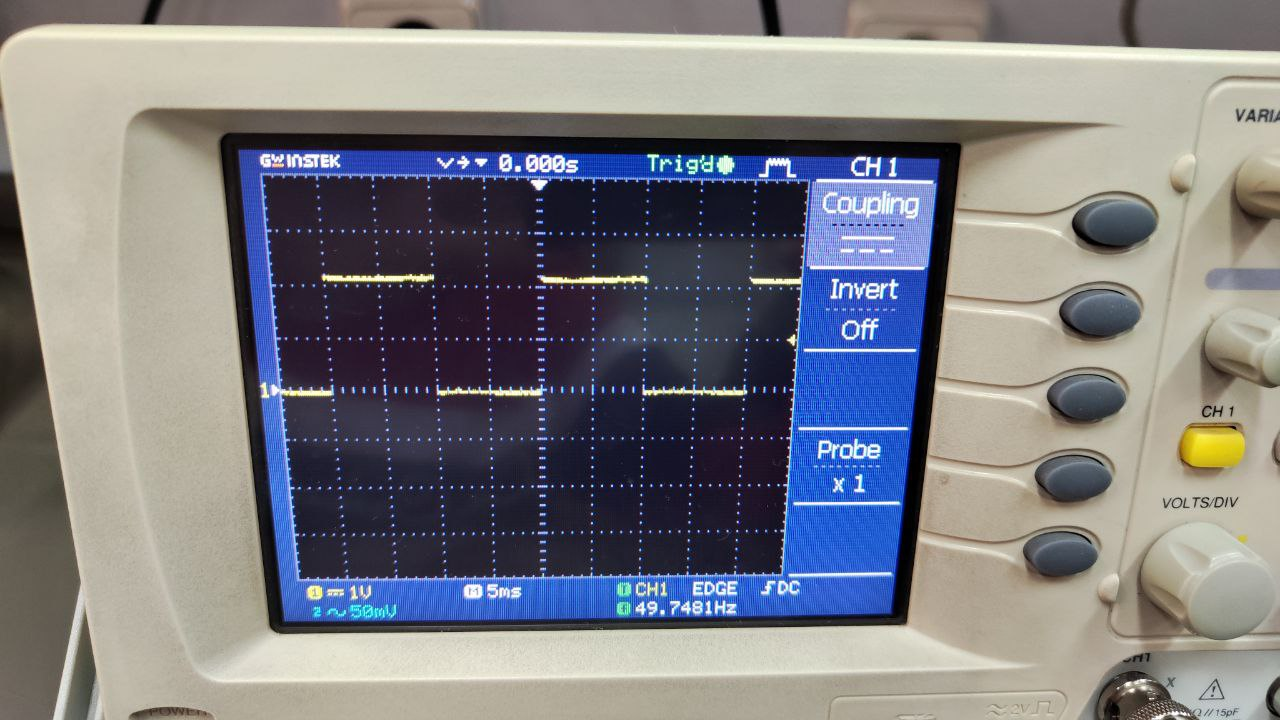
\includegraphics[scale=\PicScale]{Fig/30.jpeg}
            \caption{base wave.}
        \end{center}
    \end{figure}
    \begin{figure}[H]
        \begin{center}
            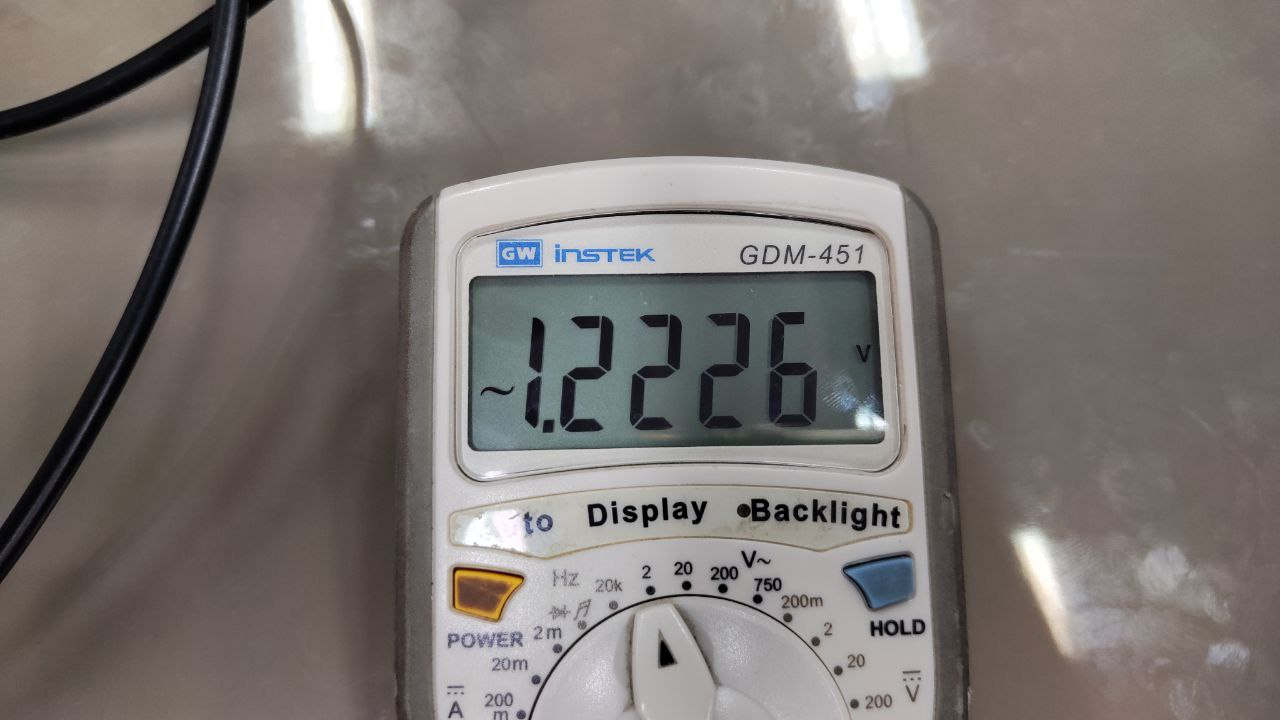
\includegraphics[scale=\PicScale]{Fig/31.jpeg}
            \caption{$V_{AC}$.}
        \end{center}
    \end{figure}

    \begin{figure}[H]
        \begin{center}
            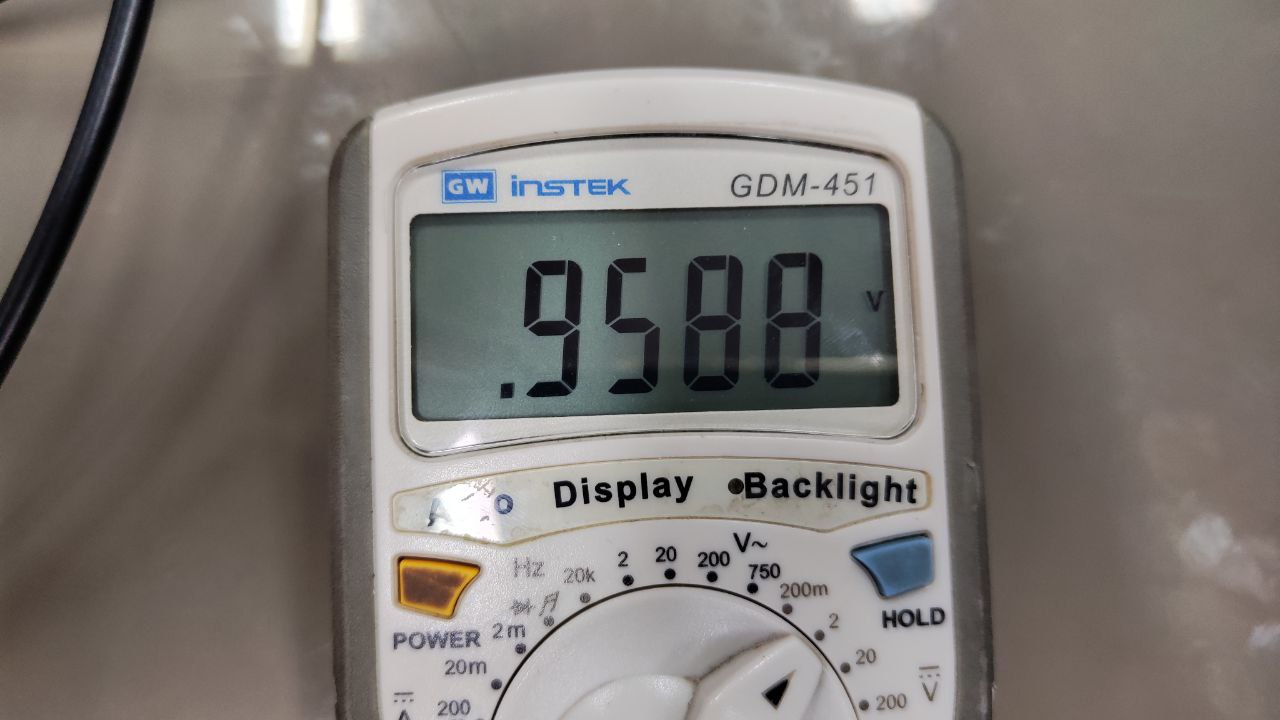
\includegraphics[scale=\PicScale]{Fig/32.jpeg}
            \caption{$V_{DC}$.}
        \end{center}
    \end{figure}

    \begin{figure}[H]
        \begin{center}
            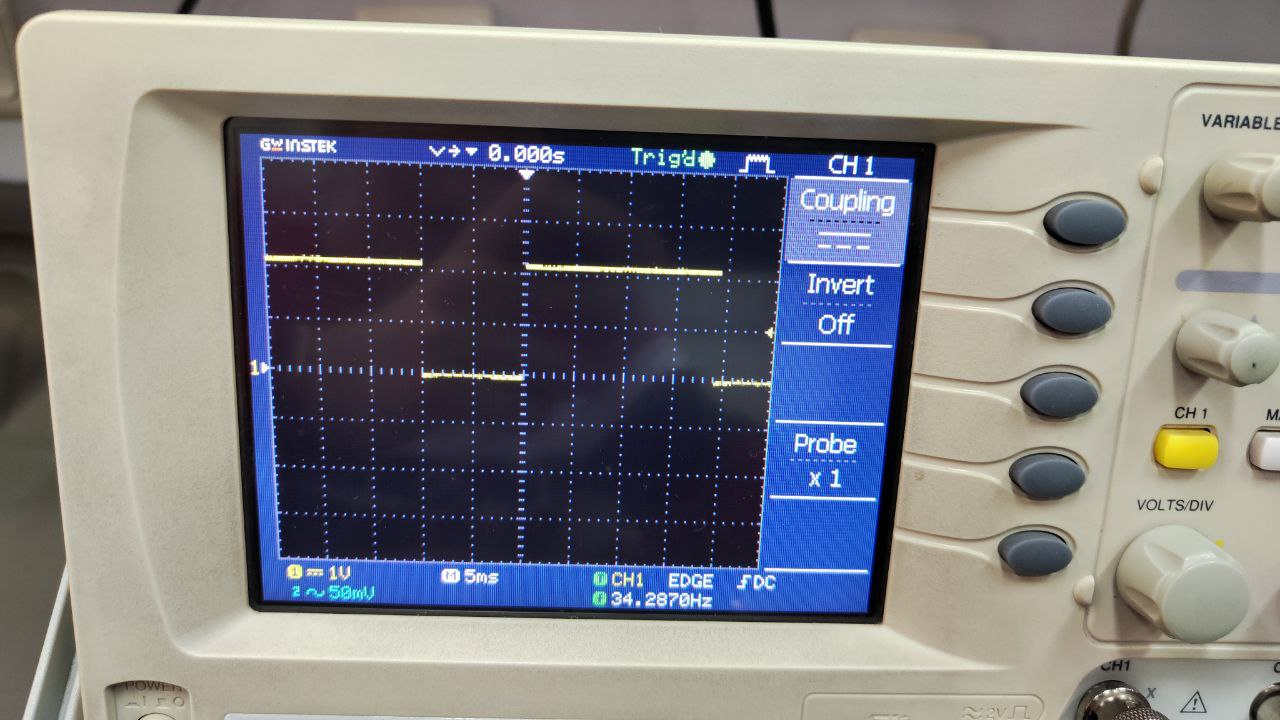
\includegraphics[scale=\PicScale]{Fig/33.jpeg}
            \caption{Duty cycle changed.}
        \end{center}
    \end{figure}
    \begin{figure}[H]
        \begin{center}
            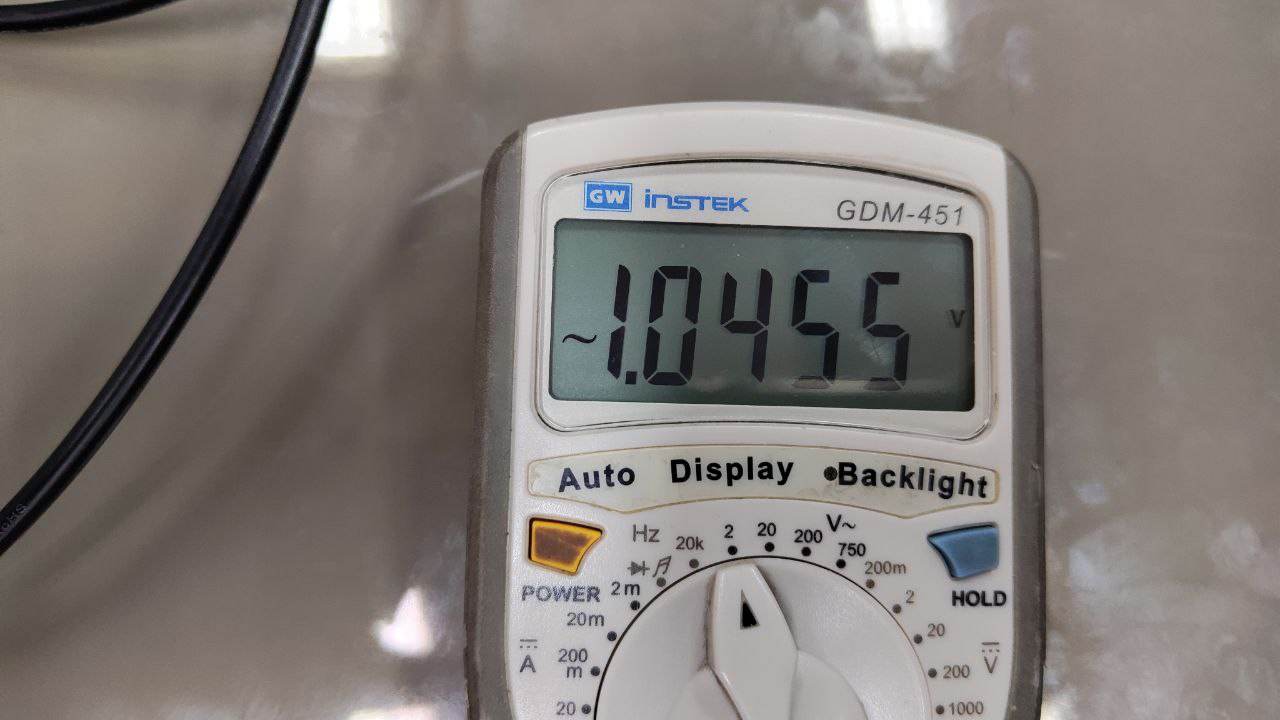
\includegraphics[scale=\PicScale]{Fig/34.jpeg}
            \caption{$V_{AC}$.}
        \end{center}
    \end{figure}

    \begin{figure}[H]
        \begin{center}
            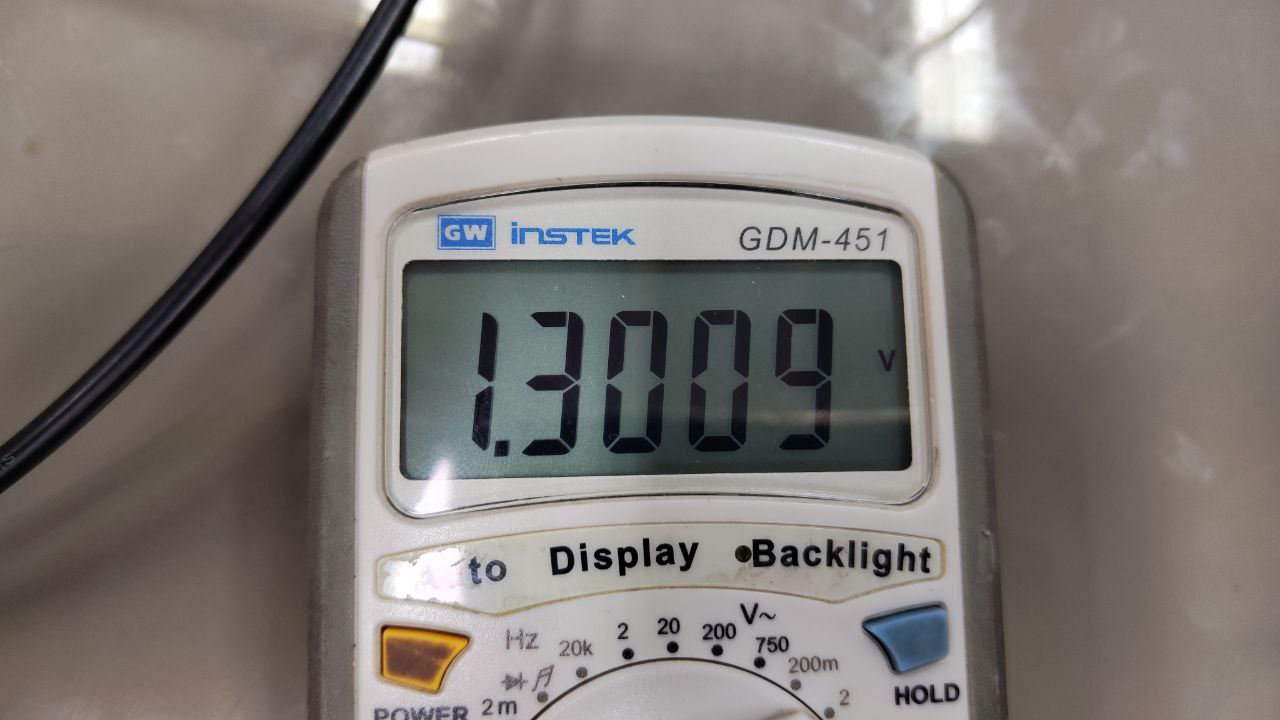
\includegraphics[scale=\PicScale]{Fig/35.jpeg}
            \caption{$V_{DC}$.}
        \end{center}
    \end{figure}
}
\end{subquestion}

\end{question}

%----------------------------------------------------------------------------------------
%	QUESTION 3
%----------------------------------------------------------------------------------------

\begin{question}

\questiontext{Tune the power supply to generate a $10$ V DC voltage on its master output.}

\begin{subquestion}{Drive a $10$ k$\Omega$ resistor with the set voltage and measure its current using the multi-meter. Compare the measured and analytical results and justify any difference.}
\answer{
    For this experiment, the current measuring module of our multimeter was burnt. So, the teacher of the second part did this experiment for everyone.
}
\end{subquestion}

\begin{subquestion}{Repeat this part for a $1$ k$\Omega$ resistor.}
\answer{
    \begin{figure}[H]
        \begin{center}
            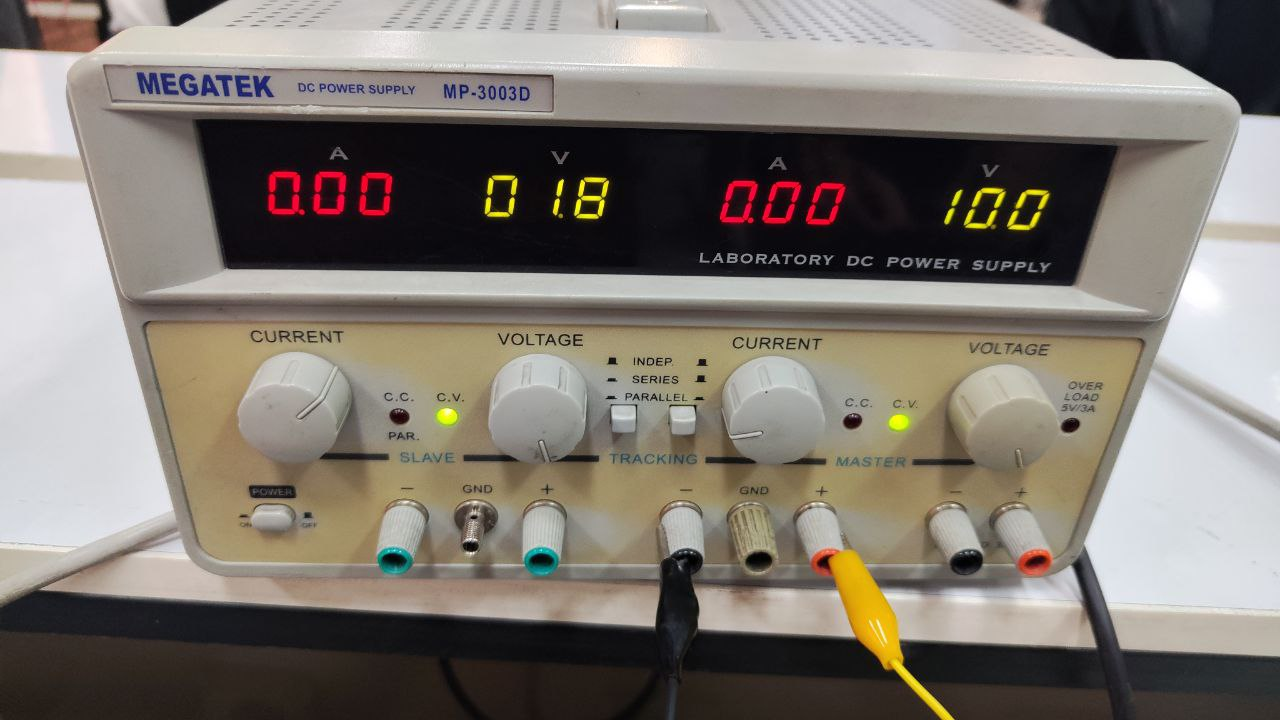
\includegraphics[scale=\PicScale]{Fig/36.jpeg}
            \caption{DC power supply.}
        \end{center}
    \end{figure}
    \begin{figure}[H]
        \begin{center}
            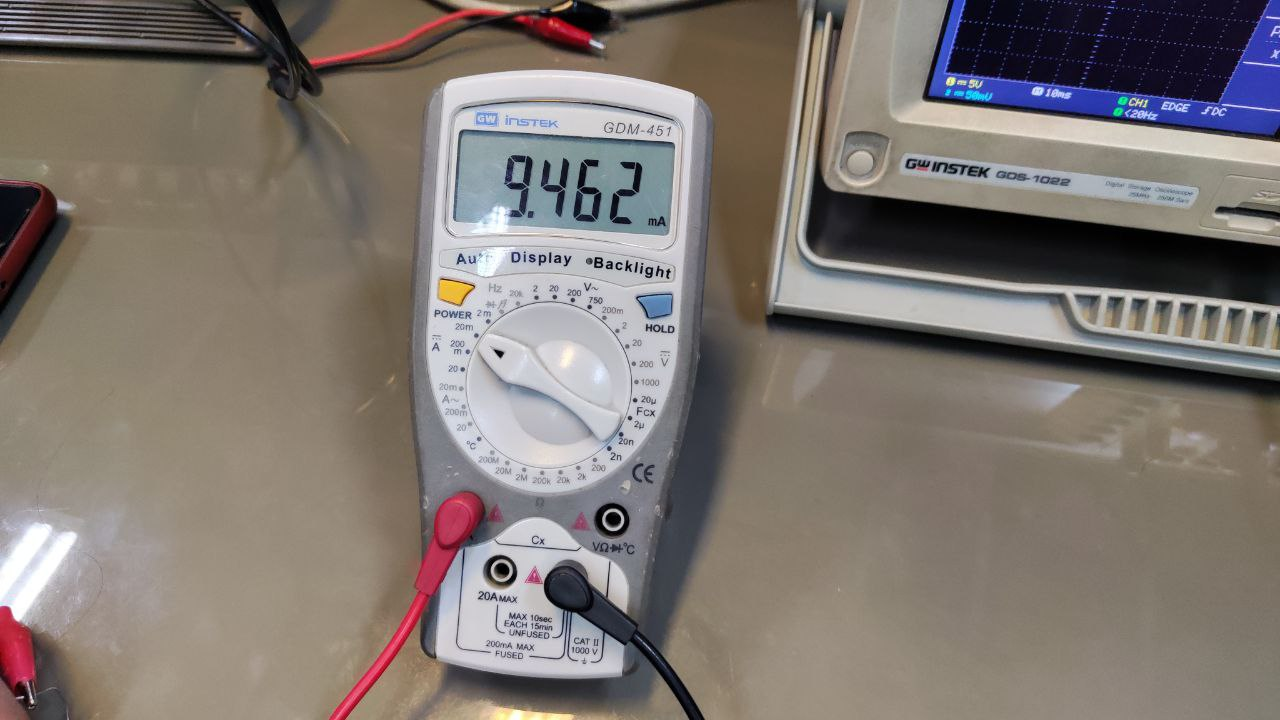
\includegraphics[scale=\PicScale]{Fig/37.jpeg}
            \caption{Current of $1$l$\Omega$ resistor.}
        \end{center}
    \end{figure}
}
\end{subquestion}

\end{question}


%----------------------------------------------------------------------------------------
%	QUESTION 4
%----------------------------------------------------------------------------------------

\begin{question}

\questiontext{Set the master output of the DC power supply to $1$ V and its corresponding current limit volume to $0$ A. Then, short circuit the master output using an alligator clip wire and turn the current volume slowly to $0.5$ A. }

\begin{subquestion}{Discuss the observations.}
\answer{
    note for my friend. This part doesn't have photo.I just have a low quality photo because this part have been done by Hadi.
}
\end{subquestion}

\begin{subquestion}{What do the C.C and C.V LEDs show?}
\answer{}
\end{subquestion}

\begin{subquestion}{Can you propose an experiment to measure the resistance of the alligator clip wire?}
\answer{}
\end{subquestion}

\end{question}

%----------------------------------------------------------------------------------------
%	QUESTION 5
%----------------------------------------------------------------------------------------

\begin{question}

\questiontext{The DC power supply has three operational modes of independent, series, and parallel.}

\begin{subquestion}{Use the supply to create two independent $2$ V and $3$ V DC voltages and measure them using the multi-meter.}
\answer{
    \begin{figure}[H]
        \begin{center}
            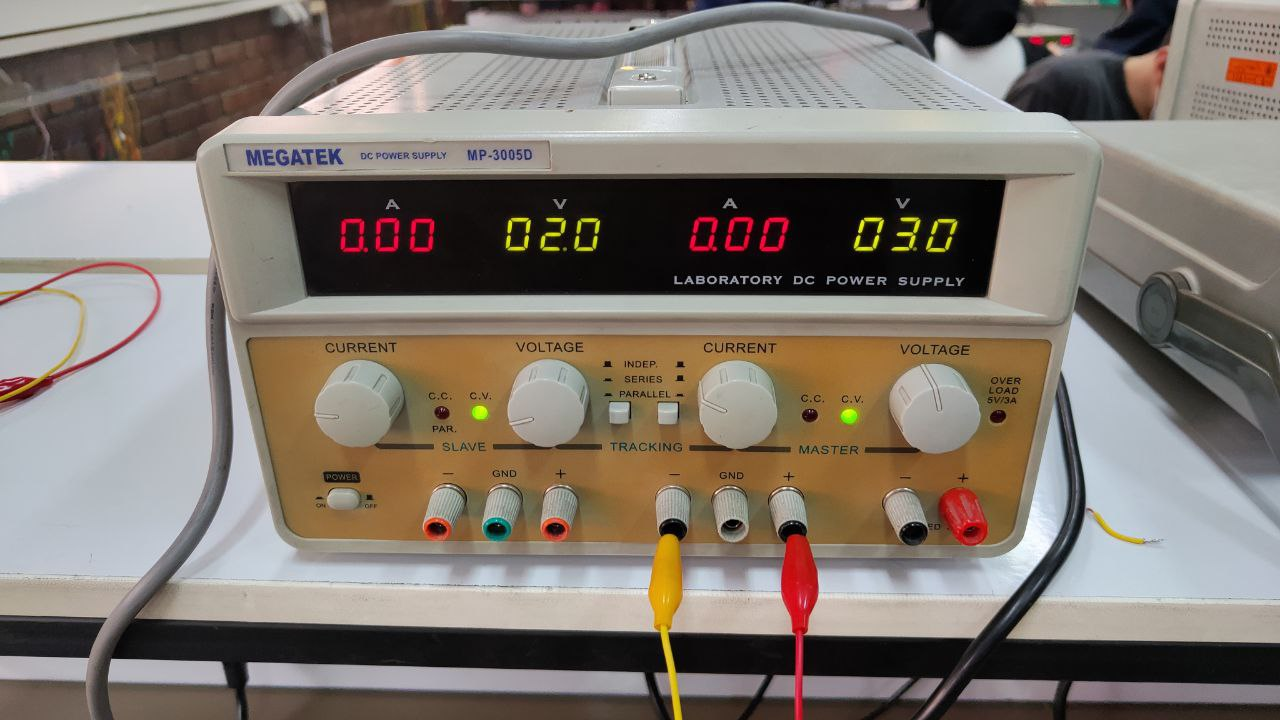
\includegraphics[scale=\PicScale]{Fig/38.jpeg}
            \caption{DC power supply setup.}
        \end{center}
    \end{figure}

    \begin{figure}[H]
        \begin{center}
            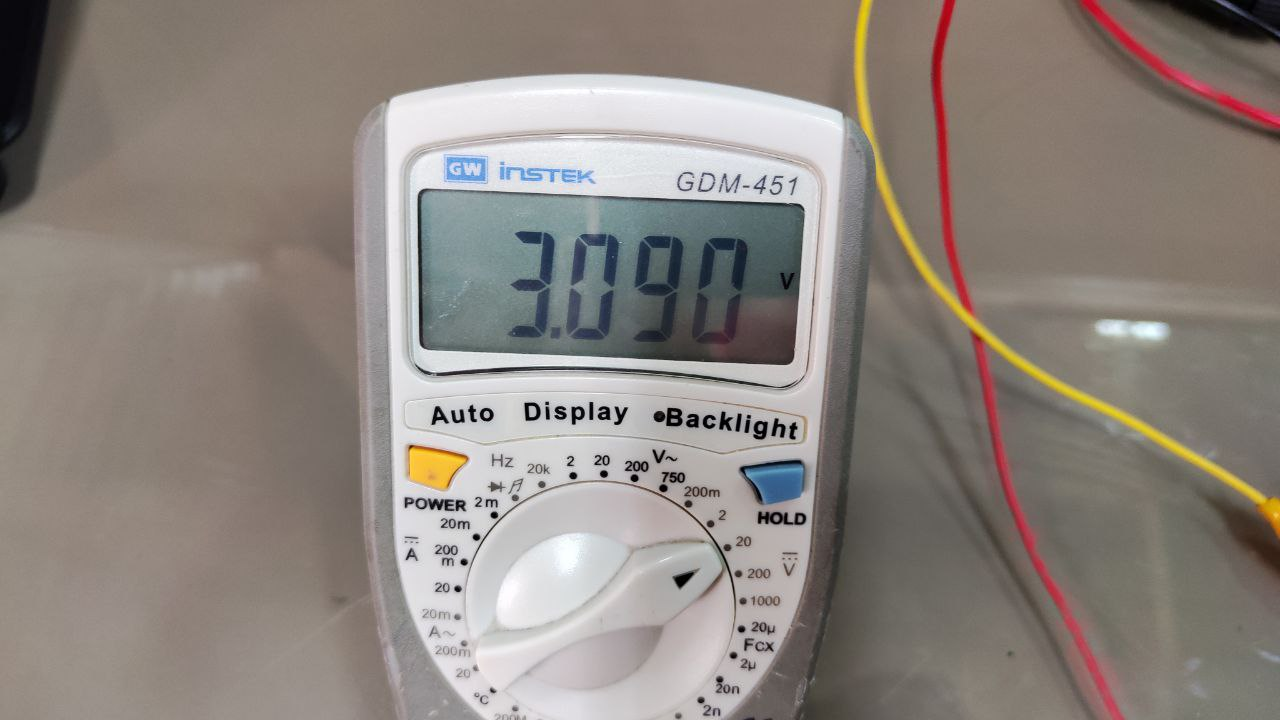
\includegraphics[scale=0.1]{Fig/39.jpeg}
            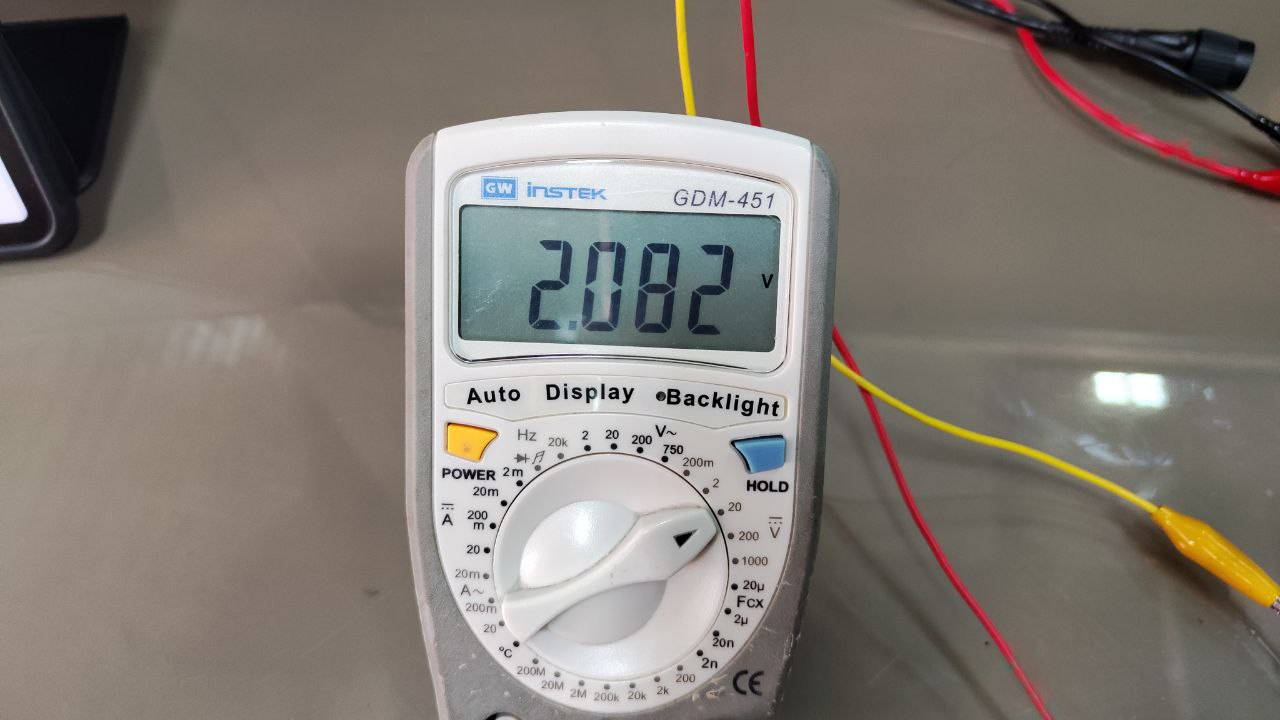
\includegraphics[scale=0.1]{Fig/40.jpeg}
            \caption{Multimeter.}
        \end{center}
    \end{figure}
}
\end{subquestion}

\begin{subquestion}{Use the supply in parallel mode to create a $3$ V DC voltage and measure it using the multi-meter. How is this voltage different from a $3$ V voltage generated from the master output on independent mode?}
\answer{
    \begin{figure}[H]
        \begin{center}
            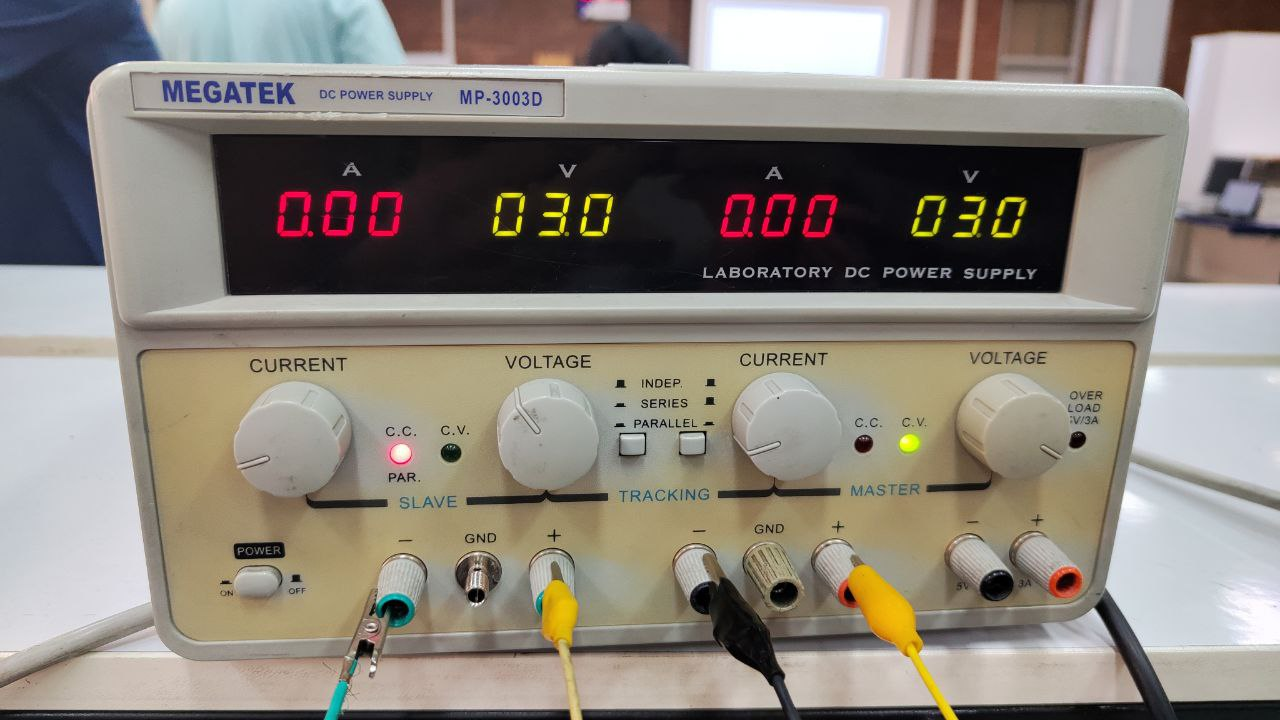
\includegraphics[scale=\PicScale]{Fig/41.jpeg}
            \caption{DC power supply setup.}
        \end{center}
    \end{figure}

    \begin{figure}[H]
        \begin{center}
            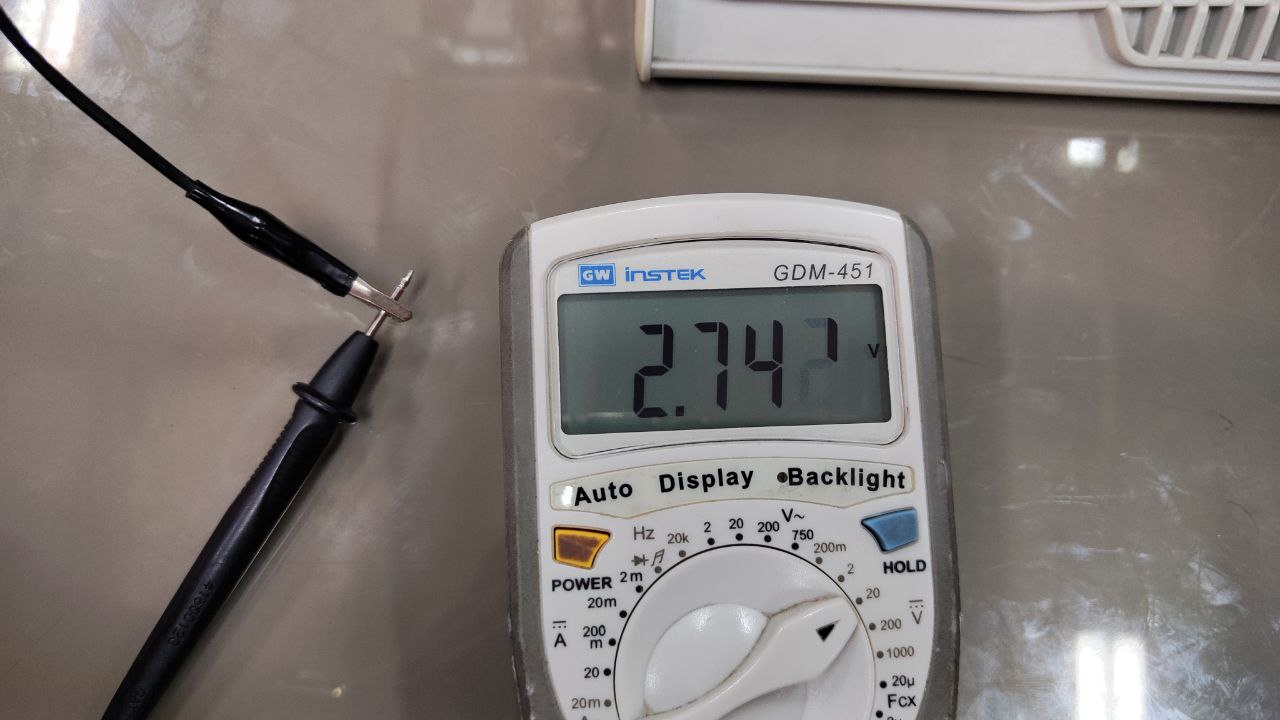
\includegraphics[scale=\PicScale]{Fig/42.jpeg}
            \caption{Multimeter for both outputs.}
        \end{center}
    \end{figure}
}
\end{subquestion}

\begin{subquestion}{Use the supply in series mode to create two $\pm 2$ V DC voltages and measure them using the multi-meter.}
\answer{
    \begin{figure}[H]
        \begin{center}
            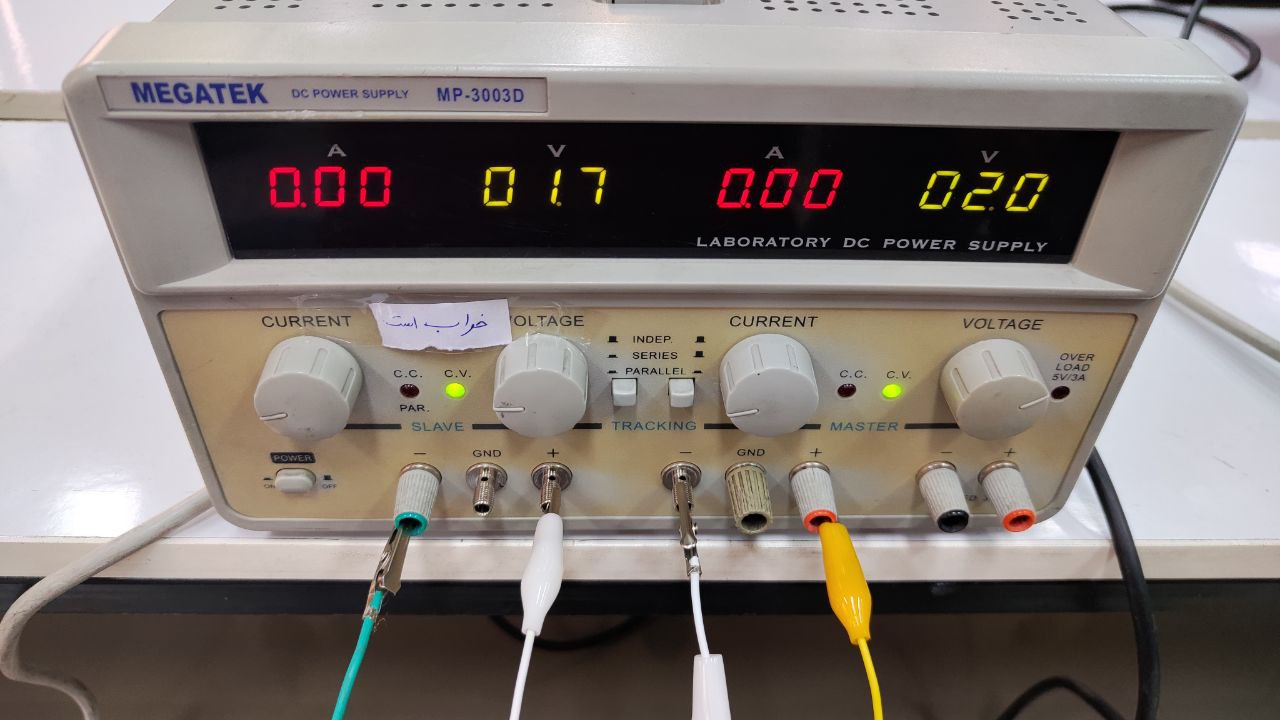
\includegraphics[scale=\PicScale]{Fig/43.jpeg}
            \caption{DC power supply setup.}
        \end{center}
    \end{figure}

    \begin{figure}[H]
        \begin{center}
            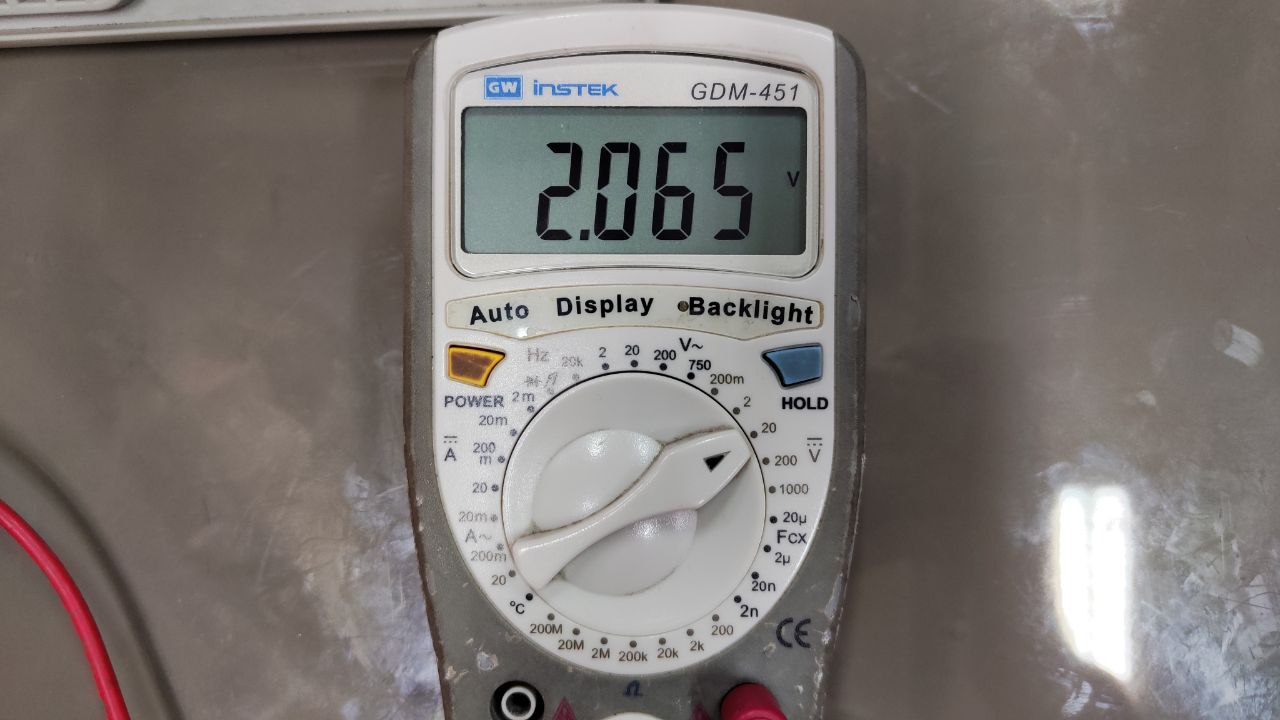
\includegraphics[scale=0.1]{Fig/44.jpeg}
            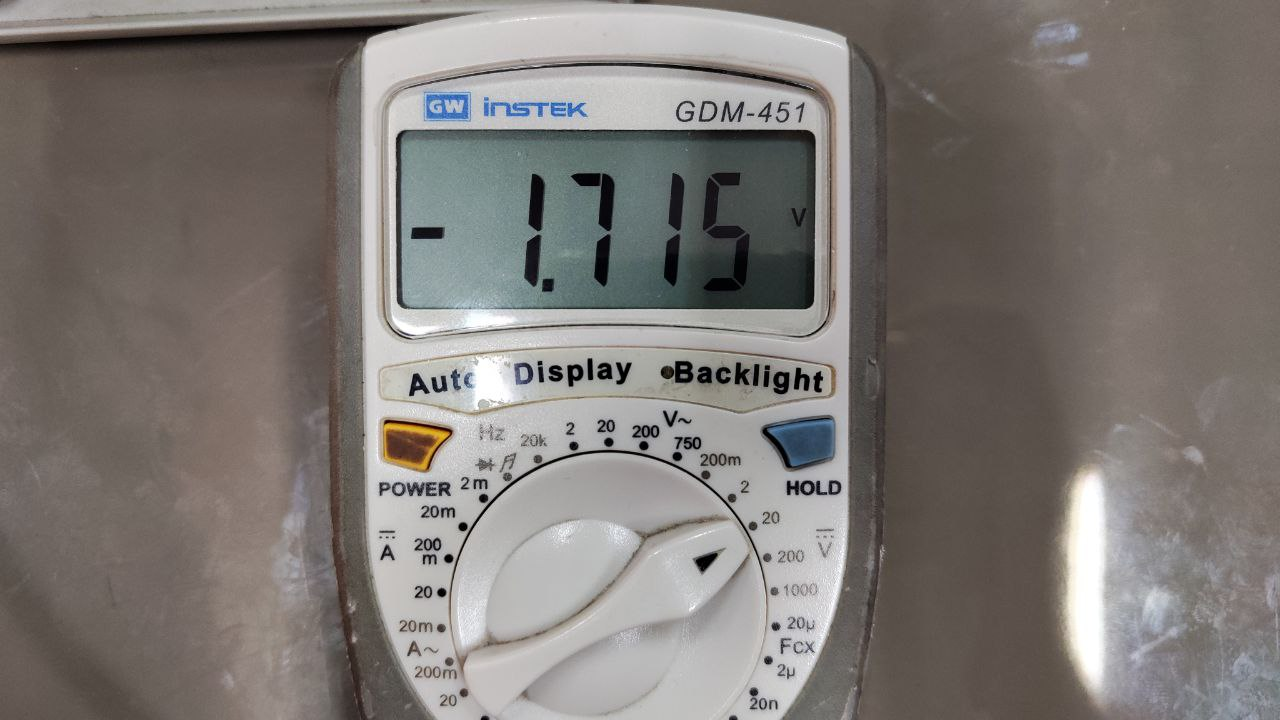
\includegraphics[scale=0.1]{Fig/45.jpeg}
            \caption{Multimeter.}
        \end{center}
    \end{figure}
}
\end{subquestion}

\begin{subquestion}{Use the supply to create two $-2$ V and $3$ V DC voltages and measure them using the multi-meter.}
\answer{
    \begin{figure}[H]
        \begin{center}
            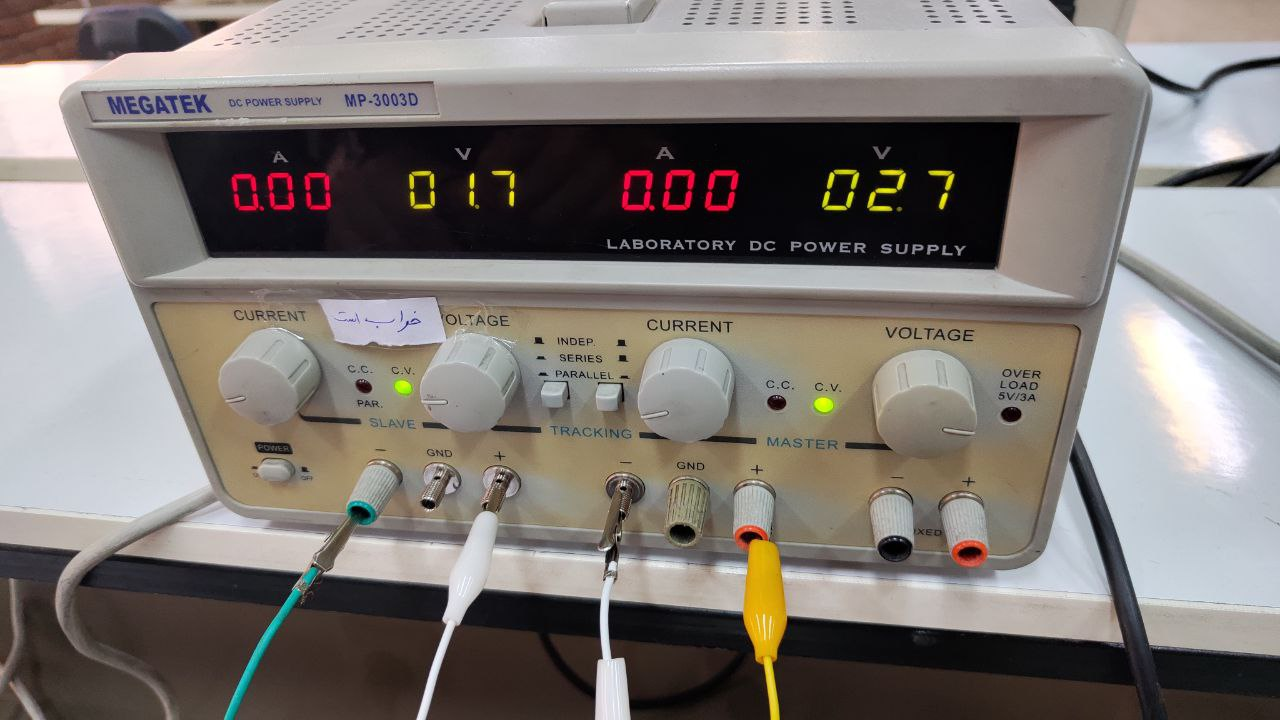
\includegraphics[scale=\PicScale]{Fig/46.jpeg}
            \caption{DC power supply setup.}
        \end{center}
    \end{figure}

    \begin{figure}[H]
        \begin{center}
            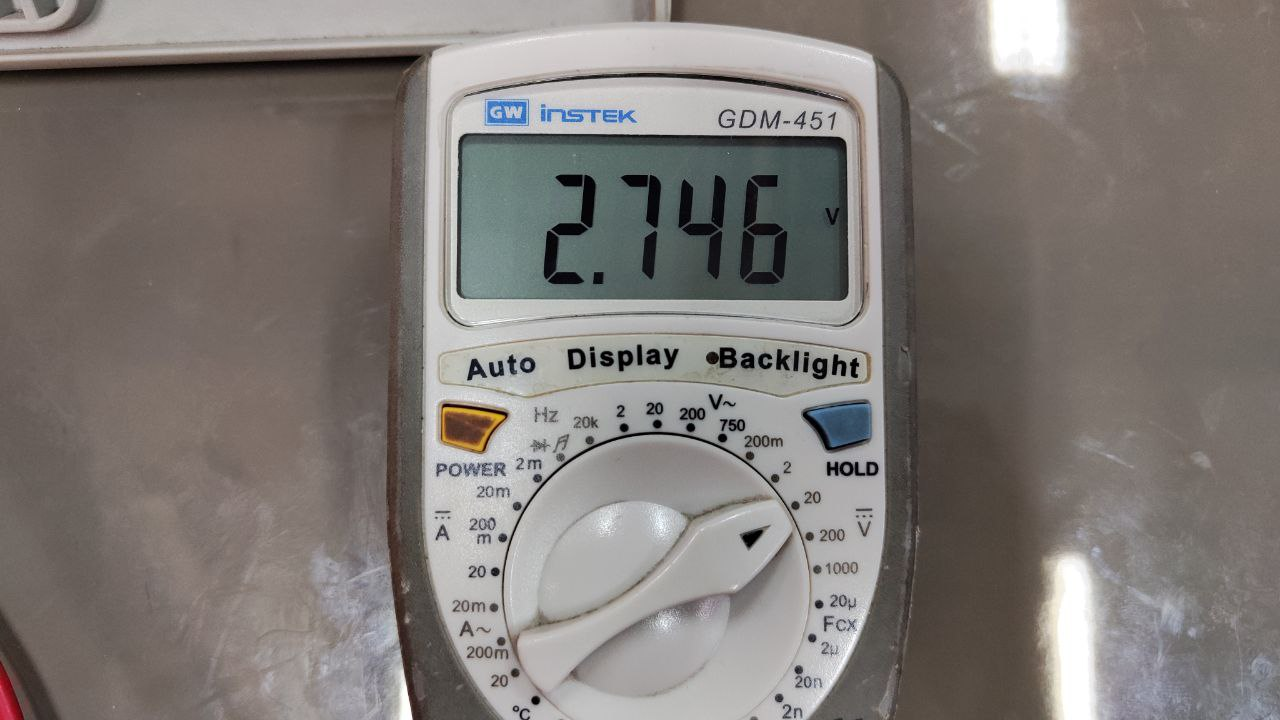
\includegraphics[scale=0.1]{Fig/47.jpeg}
            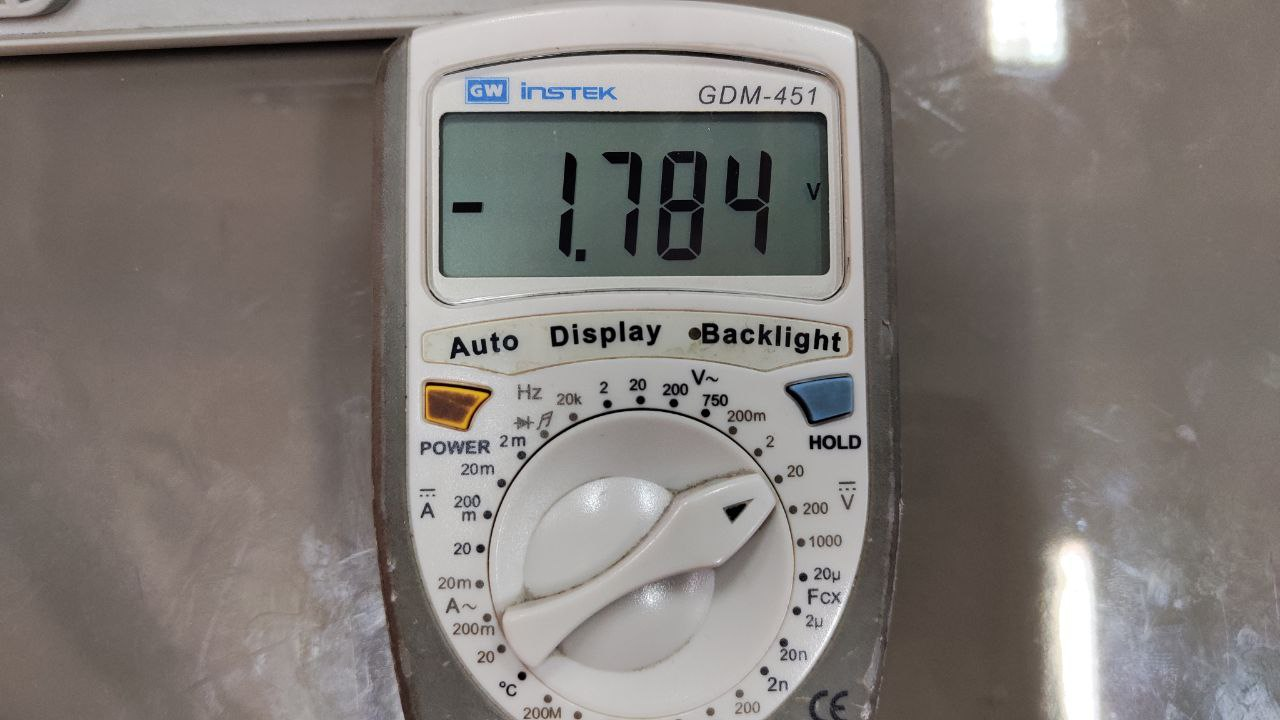
\includegraphics[scale=0.1]{Fig/48.jpeg}
            \caption{Multimeter.}
        \end{center}
    \end{figure}
}
\end{subquestion}

\end{question}


%----------------------------------------------------------------------------------------
%	QUESTION 6
%----------------------------------------------------------------------------------------

\begin{question}

\questiontext{Set the selector dial of the multi-meter to resistance mode.}

\begin{subquestion}{Measure the resistance of a $1$ k$\Omega$ resistor in the most accurate range and compare it with the nominal resistance value.}
\answer{
    \begin{figure}[H]
        \begin{center}
            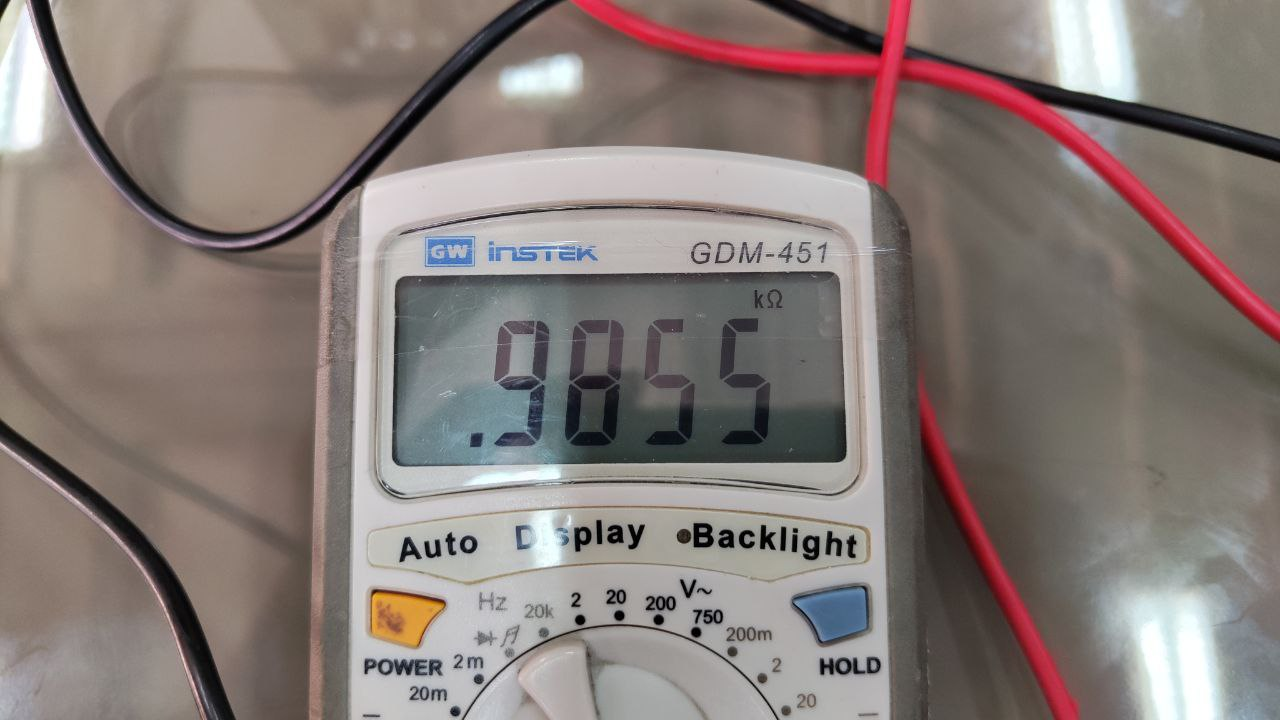
\includegraphics[scale=\PicScale]{Fig/49.jpeg}
            \caption{Multimeter.}
        \end{center}
    \end{figure}
    The difference is because of resistor error.
}
\end{subquestion}

\begin{subquestion}{Repeat the previous part for a $100$ k$\Omega$ resistor. What happens if you touch the probes of the multi-meter while measuring the resistance?}
\answer{
    \begin{figure}[H]
        \begin{center}
            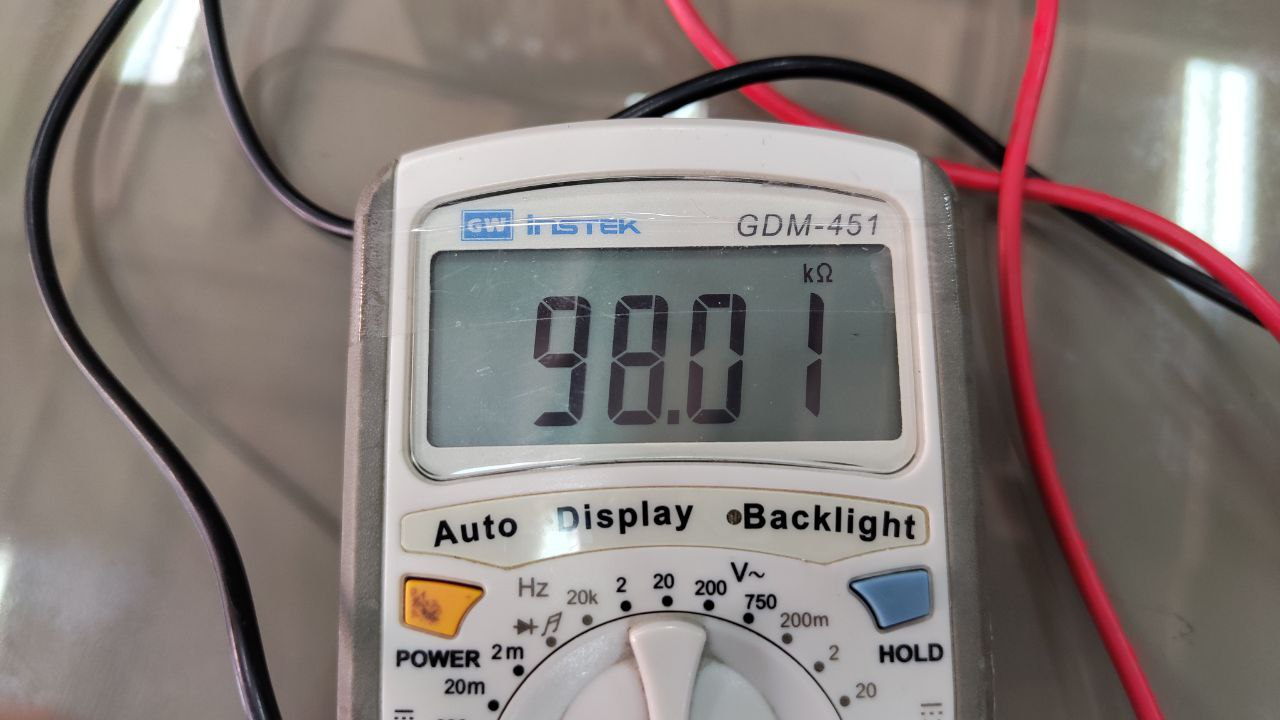
\includegraphics[scale=\PicScale]{Fig/50.jpeg}
            \caption{Multimeter.}
        \end{center}
    \end{figure}

    \begin{figure}[H]
        \begin{center}
            \includegraphics[scale=\PicScale]{Fig/51.jpeg}
            \caption{touching the probes of the multi-meter while measuring the resistance.}
        \end{center}
    \end{figure}
}
\end{subquestion}

\begin{subquestion}{Connect the probes of the multi-meter to each other and read the displayed resistance. Can you measure the resistance of an alligator clip wire using the multi-meter and its probes? }
\answer{
    \begin{figure}[H]
        \begin{center}
            \includegraphics[scale=\PicScale]{Fig/52.jpeg}
            \caption{Multimeter initial resistor.}
        \end{center}
    \end{figure}

    \begin{figure}[H]
        \begin{center}
            \includegraphics[scale=\PicScale]{Fig/53.jpeg}
            \caption{Multimeter measuring the resistance of an alligator clip wire.}
        \end{center}
    \end{figure}

    \begin{figure}[H]
        \begin{center}
            \includegraphics[scale=\PicScale]{Fig/54.jpeg}
            \caption{setup for measuring the resistance of an alligator clip wire.}
        \end{center}
    \end{figure}
}
\end{subquestion}

\end{question}


%----------------------------------------------------------------------------------------
%	QUESTION 7
%----------------------------------------------------------------------------------------

\begin{question}

\questiontext{Set the selector dial of the multi-meter to continuity test mode.}

\begin{subquestion}{Connect the probes of the multi-meter to a $10$ k$\Omega$ resistor and see what happens.}
\answer{
    \begin{figure}[H]
        \begin{center}
            \includegraphics[scale=\PicScale]{Fig/55.jpeg}
            \caption{Multimeter.}
        \end{center}
    \end{figure}
}
\end{subquestion}


\begin{subquestion}{Repeat the previous part for a $1$ k$\Omega$ resistor and for short-circuited probes.}
\answer{
    \begin{figure}[H]
        \begin{center}
            \includegraphics[scale=\PicScale]{Fig/56.jpeg}
            \caption{Multimeter.}
        \end{center}
    \end{figure}
}
\end{subquestion}

\begin{subquestion}{Can you determine the threshold value of the continuity test mode using a simple experiment?}
\answer{
    \begin{figure}[H]
        \begin{center}
            \includegraphics[scale=\PicScale]{Fig/57.jpeg}
            \caption{Approximate threshold value.}
        \end{center}
    \end{figure}
}
\end{subquestion}

\end{question}


\assignmentSection{Bonus Experiments}

%----------------------------------------------------------------------------------------
%	QUESTION 8
%----------------------------------------------------------------------------------------

\begin{question}

\questiontext{How can the legs of a diode be determined using a multi-meter which has no diode test feature?}

\answer{}

\end{question}

%----------------------------------------------------------------------------------------
%	QUESTION 9
%----------------------------------------------------------------------------------------
\begin{question}
\questiontext{The DT9208 multimeter is used to measure a $5$ V DC voltage. The catalog of the multimeter is available online.
}

\begin{subquestion}{Calculate the measurement accuracy if the voltage is measured using the $20$ V range.} 
\answer{}
\end{subquestion}
%--------------------------------------------
\begin{subquestion}{Calculate the measurement accuracy if the voltage is measured using the $200$ V range.} 
\answer{}
\end{subquestion}

%--------------------------------------------
\begin{subquestion}{Calculate the measurement accuracy if the voltage is measured using the $1000$ V range.} 
\answer{}
\end{subquestion}


\end{question}

%----------------------------------------------------------------------------------------
%	QUESTION 10
%----------------------------------------------------------------------------------------

\begin{question}

\questiontext{Return your work report by filling the \LaTeX template of the manual. Include useful and high-quality images to make the report more readable and understandable.}

\end{question}

%----------------------------------------------------------------------------------------

\end{document}
